\documentclass[openary, a4paper, oneside]{jsarticle}

%%%%% 基本設定>bibのコンパイルはjbibtexで %%%%%
% // ビルドのレシピ
% "latex-workshop.latex.recipes": [
% 	{
% 			"name": "toolchain",
% 			"tools": [
% 					"Step 1: ptex2pdf",
% 					"Step 1: ptex2pdf",
% 					//"Step 2: pbibtex",
% 					"Step 2: jbibtex",
% 					"Step 3: ptex2pdf",
% 					"Step 4: ptex2pdf",
% 			]
% 	}
% ],
%%%%%%%%%%%%%%%%%%%%%%%%%%%%%%%%%%%%%%%%%%%%


\usepackage[top=10truemm,bottom=20truemm,left=15truemm,right=15truemm]{geometry}
\usepackage[T1]{fontenc}
\usepackage[dvipdfmx]{hyperref, graphicx, color}
\usepackage{atbegshi}

\ifnum 42146=\euc"A4A2
\AtBeginShipoutFirst{\special{pdf:tounicode EUC-UCS2}}
\else
\AtBeginShipoutFirst{\special{pdf:tounicode 90ms-RKSJ-UCS2}}
\fi
\usepackage[all]{xy}
\usepackage{makeidx}

\makeindex

\usepackage{url}
\usepackage{eucal}
\usepackage{amsthm}
\usepackage{amsmath}
\usepackage{amssymb}
\usepackage{amsfonts}
\usepackage{mathrsfs}
\usepackage{wasysym}
\usepackage{bm}
\usepackage{color}
\usepackage{comment}			% コメント関数
%\usepackage{udline}					% 行をまたいだ下線(\ul{ })
\usepackage{ascmac}				% 複数行を枠で囲む eg. \begin{itembox}[位置]{題}...\end{itembox}

\usepackage{tikz}
\usetikzlibrary{positioning}

\bibliographystyle{jplain}
\addtolength{\footskip}{5mm}
\makeatletter
\def\ps@plainfoot{%
\let\@mkboth\@gobbletwo
\let\@oddhead\@empty
\def\@oddfoot{\normalfont\hfil-- \thepage\ --\hfil}%
\let\@evenhead\@empty
\let\@evenfoot\@oddfoot}
\let\ps@plain\ps@plainfoot

\makeatother

\pagestyle{plain}											%ページ書式


\makeatletter
\renewcommand{\theequation}{\thesection.\arabic{equation}}
\@addtoreset{equation}{section}
\makeatother
\makeatletter
\newcommand*{\defeq}{\mathrel{\rlap{%
\raisebox{0.3ex}{$\m@th\cdot$}}%
\raisebox{-0.3ex}{$\m@th\cdot$}}%

=}

\newcommand*{\eqdef}{=\mathrel{\hbox to 0pt{%
\raisebox{0.3ex}{$\m@th\cdot$}}%
\raisebox{-0.3ex}{$\m@th\cdot$}}%

}

\makeatother



\DeclareMathOperator*{\slim}{s-lim}
\DeclareMathOperator*{\wlim}{w-lim}
\DeclareMathOperator{\diag}{diag}
\DeclareMathOperator{\diam}{diam}
\newcommand{\card}{\mathrm{card}\,}
\newcommand{\co}{\mathrm{co}\,}
\newcommand{\const}{\mathrm{const.}}
\newcommand{\coim}{\mathrm{Coim}\,}
\newcommand{\coker}{\mathrm{Coker}\,}
\newcommand{\dimension}{\mathrm{dim}\,}
\newcommand{\BC}{\mathrm{BC}}
\newcommand{\dom}{\mathrm{dom}\,}
\newcommand{\ind}{\mathrm{Ind}\,}
\newcommand{\Rad}{\mathrm{Rad}\,}
\newcommand{\ran}{\mathrm{ran}\,}
\newcommand{\algoplus}{\mathop{\hat{\bigoplus}}}
\newcommand{\algotimes}{\mathop{\hat{\bigotimes}}}
\newcommand{\esssup}{\mathop{\mathrm{ess.sup}}}
\DeclareMathOperator{\grad}{grad \,}
\DeclareMathOperator{\rot}{rot \,}
\DeclareMathOperator{\divergence}{div \,}
\newtheoremstyle{break}								%定理の書式(plain,break,,,)
{\topsep}{\topsep}%
{\itshape}{}%
{\bfseries}{}%
{\newline}{}%
\newtheoremstyle{breakdefn}
{\topsep}{\topsep}%
{\normalfont}{}%
{\bfseries}{}%
{\newline}{}%
\renewcommand{\proofname}{\textup{\textbf{Proof}}}		%定理系補題他
\theoremstyle{breakdefn}
\newtheorem{thm}{Theorem}[section]
\newtheorem{cor}[thm]{Corollary}
\newtheorem{lem}[thm]{Lemma}
\newtheorem{pos}[thm]{Postulate}
\newtheorem{req}[thm]{Request}
\newtheorem{prop}[thm]{Proposition}
\newtheorem{axm}[thm]{Axiom}
\newtheorem{defn}[thm]{Definition}
\newtheorem{ex}[thm]{Example}
\newtheorem{exercise}[thm]{Exercise}
\newtheorem{problem}[thm]{Problem}
\newtheorem{rem}[thm]{Remark}
\newtheorem{fact}[thm]{Fact}
\newtheorem{assump}[thm]{Assumption}
\newtheorem{notation}[thm]{Notation}
\newtheorem{claim}[thm]{Claim}

\renewcommand{\Im}{\mathrm{Im} \,}
\renewcommand{\Re}{\mathrm{Re} \,}

%%%%%%%%%%%%%%%%%%%%%%%%%%%%%%%%%%%%%%%%%%%

%%   brackets and such

%%%%%%%%%%%%%%%%%%%%%%%%%%%%%%%%%%%%%%%%%%%

\newcommand{\abs}[1]{\left|#1\right|}
\newcommand{\norm}[1]{\left\Vert#1\right\Vert}
\newcommand{\inftynorm}[1]{\left\Vert#1\right\Vert_{\infty}}
\newcommand{\pnorm}[1]{\left\Vert#1\right\Vert_p}
\newcommand{\qnorm}[1]{\left\Vert#1\right\Vert_q}
\newcommand{\twonorm}[1]{\norm{#1}_2}
\newcommand{\dbk}[1]{\left\langle #1 \right\rangle}
\newcommand{\rbk}[1]{\left (#1\right)}
\newcommand{\sqbk}[1]{\left[#1\right]}
\newcommand{\cbk}[1]{\left\{#1\right\}}
\newcommand{\abk}[1]{\left\langle #1 \right\rangle}
\newcommand{\bkt}[2]{\left\langle#1,\,#2\right\rangle}
\newcommand{\rbkt}[2]{\left ( #1,\,#2 \right)}
\newcommand{\relmiddle}[1]{\mathrel{}\middle#1\mathrel{}}
\newcommand{\set}[2]{\left\{#1 \relmiddle| #2\right\}}
\newcommand{\bra}[1]{\left\langle #1 \right|}
\newcommand{\ket}[1]{\left| #1 \right\rangle}
\newcommand{\transpose}[1]{\,^t\!{#1}}
\renewcommand{\vector}[1]{\bm{#1}}
\newcommand{\minsec}[1]{{#1}^{\circ}}

%%%%%%%%%%%%%%%%%%%%%%%%%%%%%%%%%%%%%%%%%%%

%%   special sums and such

%%%%%%%%%%%%%%%%%%%%%%%%%%%%%%%%%%%%%%%%%%%

\newcommand{\sumtwo}[2]{\mathop{\sum_{#1}}_{#2}}
\newcommand{\sumthree}[3]{\mathop{\mathop{\sum_{#1}}_{#2}}_{#3}}
\newcommand{\sumfour}[4]{\mathop{\mathop{\mathop{\sum_{#1}}_{#2}}_{#3}}_{#4}}

%%%%%%%%%%%%%%%%%%%%%%%%%%%%%%%%%%%%%%%%%%%

\newcommand{\ann}{\mathrm{Ann}\,}
\newcommand{\ass}{\mathrm{Ass}\,}
\newcommand{\Ab}{\mathbf{Ab}}
\newcommand{\bbr}{\mathbb{r}}
\newcommand{\bbA}{\mathbb{A}}
\newcommand{\bbB}{\mathbb{B}}
\newcommand{\bbC}{\mathbb{C}}
\newcommand{\bbF}{\mathbb{F}}
\newcommand{\bbH}{\mathbb{H}}
\newcommand{\bbN}{\mathbb{N}}
\newcommand{\bbQ}{\mathbb{Q}}
\newcommand{\bbR}{\mathbb{R}}
\newcommand{\bbRd}{\mathbb{R}^d}
\newcommand{\bbS}{\mathbb{S}}
\newcommand{\bbZ}{\mathbb{Z}}
\newcommand{\bbZd}{\mathbb{Z}^d}
\newcommand{\betac}{\beta_{\mathrm{c}}}
\newcommand{\blu}{\mathrm{Bl}}
\newcommand{\bs}{\blacksquare}
\newcommand{\calA}{\mathcal{A}}
\newcommand{\calB}{\mathcal{B}}
\newcommand{\calC}{\mathcal{C}}
\newcommand{\calCN}{\mathcal{C}_{N}}
\newcommand{\calCleqN}{\mathcal{C}_{\leq N}}
\newcommand{\calD}{\mathcal{D}}
\newcommand{\calE}{\mathcal{E}}
\newcommand{\calF}{\mathcal{F}}
\newcommand{\calFb}{\mathcal{F}_{\mathrm{b}}}
\newcommand{\calFbfin}{\mathcal{F}_{\mathrm{b,fin}}}
\newcommand{\calFbAW}{\calF_{\mathrm{b,ArakiWoods}}}
\newcommand{\calFfAW}{\calF_{\mathrm{f,ArakiWyss}}}
\newcommand{\calFAW}{\calF_{\mathrm{AW}}}
\newcommand{\calFf}{\mathcal{F}_{\mathrm{f}}}
\newcommand{\calH}{\mathcal{H}}
\newcommand{\calI}{\mathcal{I}}
\newcommand{\calK}{\mathcal{K}}
\newcommand{\calL}{\mathcal{L}}
\newcommand{\calV}{\mathcal{V}}
\newcommand{\calM}{\mathcal{M}}
\newcommand{\calO}{\mathcal{O}}
\newcommand{\calR}{\mathcal{R}}
\newcommand{\calS}{\mathcal{S}}
\newcommand{\calW}{\mathcal{W}}
\newcommand{\catT}{\mathbf{T}}
\newcommand{\Cc}{C_{\mathrm{c}}}
\newcommand{\Ccinfty}{\Cc^{\infty}}
\newcommand{\cech}{\check{\mathrm{H}}}
\newcommand{\ch}{\mathbf{Ch}}
\newcommand{\chb}{\mathbf{Ch}^{\mathrm{b}}}
\newcommand{\chminus}{\mathbf{Ch}^{-}}
\newcommand{\chnonnegative}{\mathbf{Ch}^{\geq 0}}
\newcommand{\chplus}{\mathbf{Ch}^{+}}
\newcommand{\coho}{\mathrm{H}}
\newcommand{\Cov}[1]{\mathrm{Cov}\sqbk{#1}}
\newcommand{\divcl}{\mathrm{DivCl}\,}
\newcommand{\divs}{\mathrm{Div}\,}
\newcommand{\E}[1]{\rmE\sqbk{#1}}
\newcommand{\edivs}{\mathrm{Div}_+\,}
\newcommand{\EleqN}{E_{\leq}(N)}
\newcommand{\End}{\mathrm{End}}
\newcommand{\extbbC}{\overline{\bbC}}
\newcommand{\fin}{\hfill $\square$ \par}
\newcommand{\fraka}{\mathfrak{a}}
\newcommand{\frakb}{\mathfrak{b}}
\newcommand{\frakc}{\mathfrak{c}}
\newcommand{\frakd}{\mathfrak{d}}
\newcommand{\frake}{\mathfrak{e}}
\newcommand{\frakf}{\mathfrak{f}}
\newcommand{\frakg}{\mathfrak{g}}
\newcommand{\frakh}{\mathfrak{h}}
\newcommand{\fraki}{\mathfrak{i}}
\newcommand{\frakj}{\mathfrak{j}}
\newcommand{\frakk}{\mathfrak{k}}
\newcommand{\frakl}{\mathfrak{l}}
\newcommand{\frakm}{\mathfrak{m}}
\newcommand{\frakn}{\mathfrak{n}}
\newcommand{\frako}{\mathfrak{o}}
\newcommand{\frakp}{\mathfrak{p}}
\newcommand{\frakq}{\mathfrak{q}}
\newcommand{\frakr}{\mathfrak{r}}
\newcommand{\fraks}{\mathfrak{s}}
\newcommand{\frakt}{\mathfrak{t}}
\newcommand{\fraku}{\mathfrak{u}}
\newcommand{\frakv}{\mathfrak{v}}
\newcommand{\frakw}{\mathfrak{w}}
\newcommand{\frakx}{\mathfrak{x}}
\newcommand{\fraky}{\mathfrak{y}}
\newcommand{\frakz}{\mathfrak{z}}
\newcommand{\frakA}{\mathfrak{A}}
\newcommand{\frakB}{\mathfrak{B}}
\newcommand{\frakC}{\mathfrak{C}}
\newcommand{\frakD}{\mathfrak{D}}
\newcommand{\frakE}{\mathfrak{E}}
\newcommand{\frakF}{\mathfrak{F}}
\newcommand{\frakG}{\mathfrak{G}}
\newcommand{\frakH}{\mathfrak{H}}
\newcommand{\frakI}{\mathfrak{I}}
\newcommand{\frakJ}{\mathfrak{J}}
\newcommand{\frakK}{\mathfrak{K}}
\newcommand{\frakL}{\mathfrak{L}}
\newcommand{\frakM}{\mathfrak{M}}
\newcommand{\frakN}{\mathfrak{N}}
\newcommand{\frakO}{\mathfrak{O}}
\newcommand{\frakP}{\mathfrak{P}}
\newcommand{\frakQ}{\mathfrak{Q}}
\newcommand{\frakR}{\mathfrak{R}}
\newcommand{\frakS}{\mathfrak{S}}
\newcommand{\frakT}{\mathfrak{T}}
\newcommand{\frakU}{\mathfrak{U}}
\newcommand{\frakV}{\mathfrak{V}}
\newcommand{\frakW}{\mathfrak{W}}
\newcommand{\frakX}{\mathfrak{X}}
\newcommand{\frakY}{\mathfrak{Y}}
\newcommand{\frakZ}{\mathfrak{Z}}
\newcommand{\Frac}{\mathrm{Frac}\,}
\newcommand{\free}{\mathrm{fr}}
\newcommand{\Grp}{\mathbf{Grp}}
\newcommand{\He}{H_{\mathrm{e}}}
\newcommand{\Hb}{H_{\mathrm{b}}}
\newcommand{\HI}{H_{\mathrm{I}}}
\newcommand{\Hom}{\mathrm{Hom} \,}
\newcommand{\homo}{\mathrm{Hom}}
\newcommand{\hyperbolicsegment}[2]{\left[ #1, \, #2 \right]_{\mathrm{h}}}
\newcommand{\hyphen}{\mathchar`-}
\newcommand{\id}{\mathrm{id}}
\newcommand{\injsh}{\mathcal{I}}
\newcommand{\Int}{\mathrm{Int} \,}
\newcommand{\Isom}{\mathrm{Isom} \,}
\newcommand{\gvarepsilonminus}{g_{\varepsilon}^{-}}
\newcommand{\gvarepsilonplus}{g_{\varepsilon}^{+}}
\newcommand{\image}{\mathrm{Im}\,}
\newcommand{\limjtoinfty}{\lim_{j \to \infty}}
\newcommand{\liminfntoinfty}{\liminf_{n \to \infty}}
\newcommand{\limntoinfty}{\lim_{n \to \infty}}
\newcommand{\limsupntoinfty}{\limsup_{n \to \infty}}
\newcommand{\kernel}{\mathrm{Ker}\,}
\newcommand{\Le}{L_{\mathrm{e}}}
\newcommand{\Lb}{L_{\mathrm{b}}}
\newcommand{\LI}{L_{\mathrm{I}}}
\newcommand{\Loneloc}{L_{\mathrm{loc}}^1}
\newcommand{\LtwoRd}{L^2 \rbk{\bbR^d}}
\newcommand{\LtwoRn}{L^2 \rbk{\bbR^n}}
\newcommand{\map}{\longrightarrow}
\newcommand{\meanphys}[1]{\left\langle #1 \right\rangle}
\newcommand{\Mod}{\mathbf{Mod}}
\newcommand{\modr}{\Mod \mathchar`- R}
\newcommand{\obj}{\mathrm{obj}\,}
\newcommand{\OmegaAW}{\Omega_{\mathrm{AW}}}
\newcommand{\Omegab}{\Omega_{\mathrm{b}}}
\newcommand{\opposite}{\mathrm{op}}
\newcommand{\pdivs}{\mathrm{Div}_{\mathrm{princ}}\,}
\newcommand{\phirhol}{\phi_{\rho, \mathrm{l}}}
\newcommand{\pibetaAW}{\pi_{\beta}^{\mathrm{AW}}}
\newcommand{\picard}{\mathrm{Pic}\,}
\newcommand{\proj}{\mathrm{Proj}\,}
\newcommand{\rank}{\mathrm{rank} \,}
\newcommand{\realtempereddist}{\mathcal{S}'_{\mathrm{real}}}
\newcommand{\realrapiddecrease}{\mathcal{S}_{\mathrm{real}}}
\newcommand{\res}{\mathrm{Res}\,}
\newcommand{\rhoNinfty}{\rho_{N, \infty}}
\newcommand{\rhobeta}{\rho_{\beta}}
\newcommand{\riemannsphere}{\overline{\bbC}}
\newcommand{\Ring}{\mathbf{Ring}}
\newcommand{\rmod}{R \mathchar`- \Mod}
\newcommand{\rmb}{\mathrm{b}}
\newcommand{\rme}{\mathrm{e}}
\newcommand{\rmE}{\mathrm{E}}
\newcommand{\rmm}{\mathrm{m}}
\newcommand{\rmf}{\mathrm{f}}
\newcommand{\rms}{\mathrm{s}}
\newcommand{\rmirr}{\mathrm{irr}}
\newcommand{\rmirs}{\mathrm{irs}}
\newcommand{\rmfin}{\mathrm{fin}}
\newcommand{\rmas}{\mathrm{as}}
\newcommand{\rmfr}{\mathrm{fr}}
\newcommand{\rmmin}{\mathrm{min}}
\newcommand{\rmmax}{\mathrm{max}}
\newcommand{\rmtot}{\mathrm{tot}}
\newcommand{\rmg}{\mathrm{g}}
\newcommand{\rmI}{\mathrm{I}}
\newcommand{\rmIm}{\mathrm{Im}}
\newcommand{\rmRe}{\mathrm{Re}}
\newcommand{\rmp}{\mathrm{p}}
\newcommand{\rmph}{\mathrm{ph}}
\newcommand{\scrF}{\mathscr{F}}
\newcommand{\Sets}{\mathbf{Sets}}
\newcommand{\symtensor}{\bigotimes_{\mathrm{s}}}
\newcommand{\sto}{\xrightarrow{\text{s}}}
\newcommand{\sumonetoinfty}[1]{\sum_{#1 = 1}^{\infty}}
\newcommand{\sumzerotoinfty}[1]{\sum_{#1 = 0}^{\infty}}
\newcommand{\supp}{\mathrm{supp} \,}
\newcommand{\Trace}{\mathrm{Tr}}
\newcommand{\Top}{\mathbf{Top}}
\newcommand{\touw}{\stackrel{\mathrm{uw}}{\to}\,}
\newcommand{\upbf}[1]{\textup{\textbf{#1}}}
\newcommand{\VC}{V_{\mathrm{C}}}
\newcommand{\wick}[1]{\colon #1 \colon}
\newcommand{\Wrhol}{W_{\rho, \mathrm{l}}}
\newcommand{\wto}{\xrightarrow{\text{w}}}
\newcommand{\vep}{\varepsilon}
\newcommand{\sh}{\mathcal{F}}
\newcommand{\spec}{\mathrm{Spec}\,}
\newcommand{\stsh}{\mathcal{O}}
\newcommand{\Var}[1]{\mathrm{Var}\sqbk{#1}}
\bmdefine{\va}{a}
\bmdefine{\vb}{b}
\bmdefine{\vc}{c}
\bmdefine{\ve}{e}
\bmdefine{\vf}{f}
\bmdefine{\vg}{g}
\bmdefine{\vh}{h}
\bmdefine{\vi}{i}
\bmdefine{\vj}{j}
\bmdefine{\vk}{k}
\bmdefine{\vl}{l}
\bmdefine{\vm}{m}
\bmdefine{\vn}{n}
\bmdefine{\vo}{o}
\bmdefine{\vp}{p}
\bmdefine{\vq}{q}
\bmdefine{\vr}{r}
\bmdefine{\vs}{s}
\bmdefine{\vt}{t}
\bmdefine{\vu}{u}
\bmdefine{\vv}{v}
\bmdefine{\vw}{w}
\bmdefine{\vx}{x}
\bmdefine{\vy}{y}
\bmdefine{\vz}{z}
\bmdefine{\vA}{A}
\bmdefine{\vB}{B}
\bmdefine{\vC}{C}
\bmdefine{\vD}{D}
\bmdefine{\vE}{E}
\bmdefine{\vF}{F}
\bmdefine{\vG}{G}
\bmdefine{\vH}{H}
\bmdefine{\vI}{I}
\bmdefine{\vJ}{J}
\bmdefine{\vK}{K}
\bmdefine{\vL}{L}
\bmdefine{\vM}{M}
\bmdefine{\vN}{N}
\bmdefine{\vO}{O}
\bmdefine{\vP}{P}
\bmdefine{\vQ}{Q}
\bmdefine{\vR}{R}
\bmdefine{\vS}{S}
\bmdefine{\vT}{T}
\bmdefine{\vU}{U}
\bmdefine{\vV}{V}
\bmdefine{\vW}{W}
\bmdefine{\vX}{X}
\bmdefine{\vY}{Y}
\bmdefine{\vZ}{Z}

\newcommand{\an}{(a_n)_{n{\in}{\bN}}}
\newcommand{\bn}{(b_n)_{n{\in}{\bN}}}
\newcommand{\cn}{(c_n)_{n{\in}{\bN}}}
\newcommand{\xn}{(x_n)_{n{\in}{\bN}}}
\newcommand{\xm}{(x_m)_{m{\in}{\bN}}}
\newcommand{\xk}{(x_{n (k)})_{k{\in}{\bN}}}
\newcommand{\yn}{(y_n)_{n{\in}{\bN}}}
\newcommand{\fxn}{(f (x_n))_{n{\in}{\bN}}}
\newcommand{\fn}{(f_n)_{n{\in}{\bN}}}
\newcommand{\sn}{(s_n)_{n{\in}{\bN}}}
\newcommand{\pn}{(p_n)_{n{\in}{\bN}}}
\newcommand{\sgn}{\mathrm{sgn}\,}
\newcommand{\mcr}{\mathcal{R}}
\newcommand{\mcs}{\mathcal{S}}
\newcommand{\mcp}{\mathcal{P}}
\newcommand{\mcm}{\mathcal{M}}
\newcommand{\mcl}{\mathcal{L}}
\newcommand{\mcb}{\mathcal{B}}
\newcommand{\mco}{\mathcal{O}}
\newcommand{\deltat}{\varDelta t}
\newcommand{\mbr}{\mathbb{R}}
\newcommand{\mbn}{\mathbb{N}}
\newcommand{\mbz}{\mathbb{Z}}
\newcommand{\mbq}{\mathbb{Q}}
\newcommand{\mbc}{\mathbb{C}}
\newcommand{\mbfn}{\mathbf{N}}
\newcommand{\mbfz}{\mathbf{Z}}
\newcommand{\mbfq}{\mathbf{Q}}
\newcommand{\mbfr}{\mathbf{R}}
\newcommand{\mbfc}{\mathbf{C}}


\newcommand{\mrm}[1]{\mathrm{#1}}
\newcommand{\lrto}{\Longleftrightarrow}
\newcommand{\slrto}{\Longleftrightarrow}
\newcommand{\srto}{\Rightarrow}
\newcommand{\rto}{\Longrightarrow}
\newcommand{\slto}{\Leftarrow}
\newcommand{\lto}{\Longleftarrow}
\newcommand{\vecr}[3]{\rbk{#1,\quad#2,\quad#3}}
\newcommand{\vecc}[3]{\begin{pmatrix}#1\\#2\\#3\end{pmatrix}}


\newcommand{\del}{\varDelta}
\newcommand{\pd}{\partial}

\newcommand{\I}{\mathrm{i}}
\newcommand{\D}{\mathrm{d}}
\newcommand{\bbRN}{\mathbb{R}^N}
\newcommand{\Czeroinf}{C_0^{\infty}}

\newcommand{\Lone}{L^1(\Omega)}
\newcommand{\Ltwo}{L^2(\Omega)}
\newcommand{\Hone}{H^1(\Omega)}
\newcommand{\HO}{H^1_0(\Omega)}
\newcommand{\Htwo}{H^2(\Omega)}
\newcommand{\HtwoN}{H^2_N(\Omega)}
\newcommand{\Hminus}{H^{-1}(\Omega)}
\newcommand{\Hstar}{H^{1*}(\Omega)}
\newcommand{\LQ}{L^2(Q_T)}
\newcommand{\LQt}{L^2(Q_t)}
\newcommand{\LQT}{L^2(Q_T)}

\newcommand{\LoneG}{L^1(\Gamma)}
\newcommand{\LtwoG}{L^2(\Gamma)}

\newcommand{\Df}{D(f)}
\newcommand{\DF}{D(\Ftilde)}
\newcommand{\DFLO}{H}
\newcommand{\calG}{\mathcal{G}}

\newcommand{\LTLtwo}{L^2(0, T; \Ltwo)}
\newcommand{\LtLtwo}{L^2(0, t; \Ltwo)}
\newcommand{\LTHone}{L^2(0, T;\Hone)}
\newcommand{\LTHO}{L^2(0, T; \HO)}
\newcommand{\LTHtwo}{L^2(0, T; \Htwo)}
\newcommand{\LTHtwoO}{L^2(0, T; \Htwo\cap\HO)}
\newcommand{\LTHtwoN}{L^2(0, T; \HtwoN}
\newcommand{\WonetwoTLtwo}{W^{1,2}(0, T; \Lone)}
\newcommand{\HoneLtwo}{H^1(0, T; \Lone)}
\newcommand{\CTLtwo}{C([0, T]; \Lone)}
\newcommand{\CTHone}{C([0, T]; \Hone)}
\newcommand{\CTHO}{C([0, T]; \HO)}
\newcommand{\CTHtwo}{C([0, T]; \Htwo)}
\newcommand{\CTHtwoO}{C([0, T]; \Htwo\cap\HO)}
\newcommand{\ConeTLtwo}{C^1([0, T]; \Lone)}
\newcommand{\HT}{\calH_T}
\newcommand{\CdTLtwo}{C([\delta, T]; \Lone)}
\newcommand{\CeTLtwo}{C([\ve, T]; \Lone)}
\newcommand{\CopenTLtwo}{C((0, T]; \Lone)}

\newcommand{\sld}{_{\lambda}}
\newcommand{\sldk}{_{\lambda_k}}
\newcommand{\smu}{_{\mu}}
\newcommand{\smuk}{_{\mu_k}}
\newcommand{\snk}{_{n_k}}
\newcommand{\smk}{_{m_k}}
\newcommand{\salpha}{_{\alpha}}
\newcommand{\salphak}{_{\alpha_k}}
\newcommand{\sbeta}{_{\beta}}
\newcommand{\sbetak}{_{\beta_k}}
\newcommand{\sgamma}{_{\gamma}}
\newcommand{\sgammak}{_{\gamma_k}}
\newcommand{\sG}{_{\Gamma}}
\newcommand{\sS}{_{\Sigma}}
\newcommand{\sveps}{_{\veps}}

\newcommand{\Dt}{\frac{d}{dt}}
\newcommand{\Ds}{\frac{d}{ds}}
\newcommand{\dt}{\partial_t}
\newcommand{\ds}{\partial_s}
\newcommand{\dnu}{\partial_{\nu}}

\newcommand{\veps}{\varepsilon}
\newcommand{\vphi}{\varphi}
\newcommand{\vpln}{\vphi_{\lambda n}}
\newcommand{\dbeta}{1-\beta}

\newcommand{\hsum}[1]{\tilde{h}_{#1}}

\newcommand{\chara}[3]{{#1}^{\text{#2}}_{\text{#3}}}
\renewcommand{\hat}[1]{\widehat{#1}}
\renewcommand{\tilde}[1]{\widetilde{#1}}

\newcommand{\uzi}{u_{0i}}
\newcommand{\uzo}{u_{01}}
\newcommand{\uzt}{u_{02}}

\newcommand{\INTt}{\int_0^t}
\newcommand{\INTT}{\int_0^T}
\newcommand{\INTdT}{\int_{\delta}^T}
\newcommand{\INTeT}{\int_{\veps}^T}
\newcommand{\INTO}{\int_{\Omega}}
\newcommand{\INTG}{\int_{\Gamma}}

\newcommand{\CONST}{1}%%%%%%%%%%%%%%%% 仮定(A)の最良定数
\newcommand{\half}{\frac{1}{2}}

\newcommand{\fsec}{f_0}
\newcommand{\fminsec}{f^{\circ}}
\newcommand{\gsec}{g_0}
\newcommand{\fhat}{\hat{f}}
\newcommand{\ghat}{\hat{g}}
\newcommand{\Ftilde}{\tilde{F}}
\newcommand{\Gtilde}{\tilde{G}}
\newcommand{\Fbar}{\bar{F}}
\newcommand{\Gbar}{\bar{G}}
\newcommand{\phihat}{\hat{\phi}}
\newcommand{\gbar}{\bar{g}}

\newcommand{\fsecmu}{f_{0, \mu}}
\newcommand{\fsecmuk}{f_{0, \mu_k}}
\newcommand{\fsecn}{f_{0, n}}
\newcommand{\fsecnk}{f_{0, n_k}}
\newcommand{\gsecn}{g_{0, n}}
\newcommand{\gsecnk}{g_{0, n_k}}
\newcommand{\fsecnp}{f_{0, n'}}
\newcommand{\fsecnpk}{f_{0, n'_k}}
\newcommand{\gsecnp}{g_{0, n'}}
\newcommand{\gsecnpk}{g_{0, n'_k}}

\newcommand{\kt}{\tilde{k}}
\newcommand{\Kt}{\tilde{K}}
\newcommand{\htilde}{\tilde{h}}
\newcommand{\kbar}{\bar{k}}
\newcommand{\psibar}{\bar{\psi}}
\newcommand{\Cbar}{\bar{C}}
\newcommand{\Keta}{K_{\eta}}

\newcommand{\weakto}{\rightharpoonup}
\newcommand{\weakstarto}{\overset{*}{\rightharpoonup}}
\newcommand{\emb}{\hookrightarrow}
\newcommand{\emp}{\hookleftarrow}

\newcommand{\Oneln}{\text{($\ast$)$_{\lambda n}$}}
\newcommand{\Twoln}{\text{($\ast\ast$)$_{\lambda n}$}}
\newcommand{\Onel}{\text{($\ast$)$_{\lambda}$}}
\newcommand{\Twol}{\text{($\ast\ast$)$_{\lambda}$}}
\newcommand{\Onem}{\text{($\ast$)$_{\mu}$}}
\newcommand{\Twom}{\text{($\ast\ast$)$_{\mu}$}}
\newcommand{\Onen}{\text{($\ast$)$_n$}}
\newcommand{\Twon}{\text{($\ast\ast$)$_n$}}
\newcommand{\Onenp}{\text{($\ast$)$_{n'}$}}
\newcommand{\Twonp}{\text{($\ast\ast$)$_{n'}$}}
\newcommand{\Onei}{\text{($\ast$)$_i$}}
\newcommand{\Twoi}{\text{($\ast\ast$)$_i$}}
\newcommand{\Onezero}{\text{($\ast$)$_0$}}
\newcommand{\Twozero}{\text{($\ast\ast$)$_0$}}
\newcommand{\Oneone}{\text{($\ast$)$_1$}}
\newcommand{\Twoone}{\text{($\ast\ast$)$_1$}}
\newcommand{\Onetwo}{\text{($\ast$)$_2$}}
\newcommand{\Twotwo}{\text{($\ast\ast$)$_2$}}
\newcommand{\One}{\text{($\ast$)}}
\newcommand{\Two}{\text{($\ast\ast$)}}

\newcommand{\DBCIVP}{\text{(P1)}}
\newcommand{\DBCTPP}{\text{(P2)}}
\newcommand{\NBCIVP}{\text{(P3)}}
\newcommand{\NBCTPP}{\text{(P4)}}
\newcommand{\DynBCIVP}{\text{(P6)}}

\newcommand{\Aphi}{{\rm(A$\vp$)}}
\newcommand{\Aphione}{{\rm(A$\vp$-I)}}
\newcommand{\Aphitwo}{{\rm(A$\vp$-II)}}

\newcommand{\Otani}{\^Otani}
\newcommand{\Holder}{H\"older}
\newcommand{\Schrodinger}{Schr\"odinger}
\newcommand{\Arzela}{Arzel\`a}
\newcommand{\Poincare}{Poincar\'e}
\newcommand{\Komura}{K\=omura}

\title{サーベイ\\ - Cahn--Hilliard Equation with Dynamic Boundary Conditions -}
\author{Keiichiro KAGAWA}
\date{\today}

\begin{document}

\maketitle
\setcounter{tocdepth}{2}
\tableofcontents

\setcounter{section}{-1}	
\newpage
\section{文献リスト - Dynamic Boundary Condition (動的境界条件/力学的境界条件)}

\subsection{Cahn--Hilliard 方程式}

\subsubsection{混合型(GMS type)の動的境界条件}
\begin{itemize}
	\item P. Colli, G. Gilardi, and J. Sprekels, On a Cahn--Hilliard system with convection and dynamic boundary conditions, vol. 197, no. 5. Springer Berlin Heidelberg, 2018.
	\item P. Colli and T. Fukao, “Equation and dynamic boundary condition of Cahn-Hilliard type with singular potentials,” Nonlinear Anal. Theory, Methods Appl., vol. 127, pp. 413-433, 2015.
	\item G. R. Goldstein, A. Miranville, and G. Schimperna, "A Cahn–Hilliard model in a domain with non-permeable walls." Physica D: Nonlinear Phenomena 240.8 (2011): 754-766.\\
		混合型境界条件を提案.
\end{itemize}
内部でCahn--Hilliard方程式をみたし, 境界で混合型の動的境界条件をみたす問題の各論文間の関係(引用被引用関係)\\

% \begin{tikzpicture}[every node/.style={rectangle,fill=cyan!30,rounded corners}]
% 		\node (GMS) {Goldstein, Miranville, Schimperna (2011) \cite{GoldsteinMiranvilleSchimperna2011}};
% 		\node[above right=of GMS] (CF) {Colli, Fukao (2015) \cite{ColliFukao2015NA};
% 	\node[above left=of CF] (CGS) {Colli, Gilardi, Sprekels (2018) \cite{ColliGilardiSprekels2018}};

% 		\foreach \u / \v in {CF/GMS, CGS/CF, CGS/GMS}
% 				\draw[->] (\u) -- (\v);
% \end{tikzpicture}

\subsubsection{境界で Allen--Cahn 方程式を満たす動的境界条件}
\begin{itemize}
    \item L. Scarpa, “Existence and uniqueness of solutions to singular Cahn-Hilliard equations with nonlinear viscosity terms and dynamic boundary conditions,” J. Math. Anal. Appl., vol. 469, no. 2, pp. 730-764, 2019.
    \item P. Colli and T. Fukao, “Cahn-Hilliard equation with dynamic boundary conditions and mass constraint on the boundary,” J. Math. Anal. Appl., vol. 429, no. 2, pp. 1190-1213, 2015.
    \item P. Colli, M. Hassan Farshbaf-Shaker, G. Gilardi, J. Sprekels, OPTIMAL BOUNDARY CONTROL OF A VISCOUS CAHN-HILLIARD SYSTEM WITH DYNAMIC BOUNDARY CONDITION AND DOUBLE OBSTACLE POTENTIALS, SIAM J. Control Optim. 53 (2015) 2696-2721. doi:10.1007/s00245-015-9299-z.
    \item P. Colli, G. Gilardi, and J. Sprekels, “On the Cahn-Hilliard equation with dynamic boundary conditions and a dominating boundary potential,” J. Math. Anal. Appl., vol. 419, no. 2, pp. 972-994, 2014.
    \item A. Miranville, S. Zelik, The Cahn-Hilliard Equation with Singular Potentials and Dynamic Boundary Conditions, (2009) 1-37. http://arxiv.org/abs/0904.4023.
    \item A. Miranville, S. Zelik, Exponential attractors for the Cahn-Hilliard equation with dynamic boundary conditions, Math. Methods Appl. Sci. 28 (2005) 709-735. doi:10.1002/mma.590.
    \item Racke, Reinhard; Zheng, Songmu The Cahn-Hilliard equation with dynamic boundary conditions. Adv. Differential Equations 8 (2003), no. 1, 83-110.
\end{itemize}

論文の引用被引用関係(引用をしているが言及していないものは関係付けないこととする)\\

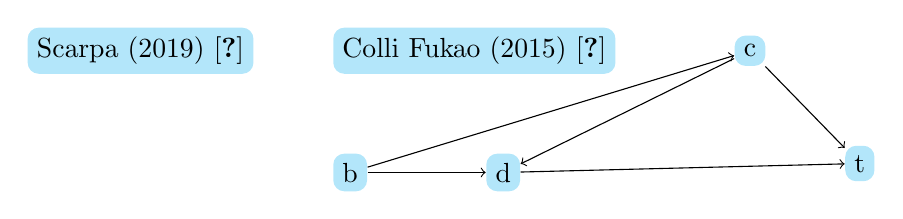
\begin{tikzpicture}[every node/.style={rectangle,fill=cyan!30,rounded corners}]
\node (S) {Scarpa (2019) \cite{Scarpa2019}};
\node[right=of S] (CF) {Colli Fukao (2015) \cite{ColliFukao2015JMAA}};
\node[below right=of S] (b) {b};
\node[right=1.5cm of CF] (c) {c};
\node[right=1.5cm of b] (d) {d};
\node[below right=of c] (t) {t};

\foreach \u / \v in {b/c,b/d,c/d,c/t,d/t}
\draw[->] (\u) -- (\v);
\end{tikzpicture}

\subsubsection{境界で Cahn--Hilliard 方程式を満たす動的境界条件}
\begin{itemize}
	\item P. Colli, T. Fukao, and H. Wu, On a transmission problem for equation and dynamic boundary condition of Cahn–Hilliard type with nonsmooth potentials, to appear in Math. Nachr.
	\item Patrik Knopf, and Kei Fong Lam. "Convergence of a Robin boundary approximation for a Cahn--Hilliard system with dynamic boundary conditions." arXiv preprint arXiv:1908.06124 (2019).
    \item C. Liu, H. Wu, “An Energetic Variational Approach for the Cahn-Hilliard Equation with Dynamic Boundary Condition: Model Derivation and Mathematical Analysis,” Arch. Rational. Mech. Anal., 233, (2019), 167-247. https://link.springer.com/article/10.1007/s00205-019-01356-x arXiv:1710.08318.
    \item H. Garcke and P. Knopf, “Weak solutions of the Cahn-Hilliard system with dynamic boundary conditions: A gradient flow approach,” vol. 1, no. 2, pp. 1-27, 2018.
    \item H. Wu, The Cahn–Hilliard equation with a new class of dynamic boundary conditions, pp. 117– 131 in “Theory of Evolution Equation and Mathematical Analysis of Nonlinear Phenomena”, RIMS K\^oky\^uroku, 2090, Kyoto University, 2018.
\end{itemize}

論文の引用被引用関係

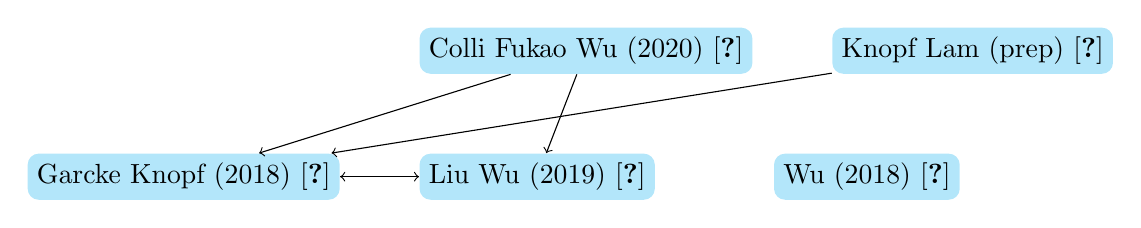
\begin{tikzpicture}[every node/.style={rectangle,fill=cyan!30,rounded corners}]
\node (GK) {Garcke Knopf (2018) \cite{GarckeKnopf2018}};
\node[right=of GK] (LW) {Liu Wu (2019) \cite{LiuWu2019}};
\node[above right=of GK] (CFW) {Colli Fukao Wu (2020) \cite{ColliFukaoWu2020}};
\node[right=1.5cm of LW] (W) {Wu (2018) \cite{Wu2018}};
\node[right=of CFW] (KL) {Knopf Lam (prep) \cite{KnopfLam2019}};

\foreach \u / \v in {GK/LW,LW/GK,CFW/GK,CFW/LW,KL/GK}
\draw[->] (\u) -- (\v);
\end{tikzpicture}

\subsection{Nonstandard Cahn--Hilliard 方程式(Podio-Guidugli type)}
\begin{itemize}
	\item P. Colli, G. Gilardi, J. Sprekels, Limiting problems for a nonstandard viscous Cahn-Hilliard system with dynamic boundary conditions, Springer INdAM Ser. 27 (2018) 217-242. doi:10.1007/978-3-319-75940-1 11.
	\item P. Colli, G. Gilardi, J. Sprekels, Global existence for a nonstandard viscous Cahn-Hilliard system with dynamic boundary condition, preprint arXiv:1608.00854 [math.AP] (2016), 1- 29.
\end{itemize}

\newpage
\section{Cahn--Hilliard 方程式 -- 混合型(GMS type)の動的境界条件}

\subsection{Colli, Gilardi, Sprekels (2018) note:19-4 pp.42-47 day:2019.08.11}
{\bf 論文情報}:
P. Colli, G. Gilardi, and J. Sprekels, On a Cahn - Hilliard system with convection and dynamic boundary conditions, vol. 197, no. 5. Springer Berlin Heidelberg, 2018.

{\bf 主問題}:
convective term($\nabla \rho \cdot u$)が含まれた viscous/pure Cahn--Hilliard 方程式を考察
混合型の動的境界条件(本論文では Cahn--Hilliard type の境界条件との記述)の下での初期値問題
\begin{equation}\nonumber\left\{\begin{aligned}
	&\dt\rho + \nabla\rho\cdot u - \Delta\mu = 0&&\text{ in }Q:=(0,T)\times\Omega,\\
	&\tau_{\Omega}\dt\rho - \Delta\rho + \beta(\rho) + \pi(\rho) \ni \mu&&\text{ in }Q,\\
	&\rho\sG = \rho|\sS, \quad \mu\sG = \mu|\sS,&&\\
	&\dt\rho\sG + \dnu\mu -\Delta\sG\mu\sG = 0&&\text{ on }\Sigma,\\
	&\tau\sG\dt\rho\sG + \dnu\rho - \Delta\sG\rho\sG + \beta\sG(\rho\sG) + \pi\sG(\rho\sG) \ni \mu\sG&&\text{ on }\Sigma,\\
	&\rho(0) = \rho_0\text{ in }\Omega\text{ and }\rho\sG(0) = \rho_0\text{ on }\Gamma.
\end{aligned}\right.\end{equation}

{\bf 先行結果}:
non convective($u=0$), pure($\tau_{\Omega}=\tau_{\Gamma}=0$) Cahn--Hilliard system
\begin{itemize}
	\item Gal(2006)\\
	Gal(2006)により導入された.
	Gal(2006)では dissipative の役割を果たし, 解の正則性を上げる$-\Delta\sG\mu\sG$の項は考えられていなかった.
	convective term($\nabla\rho\cdot u$)は問題をより複雑にする.
	\item Colli,Fukao(2015)\\
	一般のポテンシャルで弱解の存在・一意性・正則性を抽象論を用いて調べた.
	standard approximation argument に基づく.
	\item Fukao,Yamazaki(2017)\\
	最適制御問題
\end{itemize}

{\bf 新規性}:

{\bf 主結果}:

{\bf 戦略}

:

\newpage
%%%%%%%%%%%%%%%%%%%%%%%%%%%%%%%%%%%%%%%%%%%%%%%%%%%%%%%%%%%%%%%%
%%%%%%%%%%%%%%%%%%%%%%%%%%%%%%%%%%%%%%%%%%%%%%%%%%%%%%%%%%%%%%%%

\subsection{Colli, Fukao (2015) note:null day:2019.10.07}
{\bf 論文情報}:
P. Colli and T. Fukao, “Equation and dynamic boundary condition of Cahn-Hilliard type with singular potentials,” Nonlinear Anal. Theory, Methods Appl., vol. 127, 2015, pp. 413-433.

{\bf 主問題}:
\begin{equation}\left\{\begin{aligned}
	&\dt u - \Delta\mu = 0\quad\text{a.e. in }Q,\\
	&\mu = -\Delta u + \xi + \pi(u) - f, \quad \xi\in\beta(u)\quad\text{a.e. in }Q,\\
	&u\sG = u|\sG,\quad \mu\sG = \mu|\sG,\quad
	\dt u\sG + \dnu\mu - \Delta\sG\mu\sG\quad\text{a.e. on }\Sigma,\\
	&\mu\sG = \dnu u - \Delta\sG u\sG + \xi\sG + \pi\sG(u\sG) - f\sG,\quad \xi\sG\in\beta\sG(u\sG)\quad\text{a.e. on }\Sigma,\\
	&u(0) = u_0\quad \text{a.e. in }\Omega,\quad u\sG(0)=u_{0\Gamma}\quad\text{a.e. on }\Gamma. 
\end{aligned}\right. \end{equation}

この問題では次の時間に関する保存量が存在する.
\begin{equation}
	m_0 := \frac{1}{|\Omega|+|\Gamma|}\left\{ \INTO zdx + \INTG z\sG d\Gamma \right\}\quad\text{for all }\vector{z} \in \bm{H}.
\end{equation}

{\bf 先行結果}:
\begin{itemize}
	\item Colli, Fukao (2014) \cite{ColliFukao2015MMAS} 内部でAllen--Cahn, 境界でAllen--Cahn方程式をみたす動的境界問題, 本論文と同様の手法を用いているので参考になる.
\end{itemize}

{\bf 新規性}:

{\bf 主結果}:
条件(A1)-(A4)で弱解の初期値-外力連続依存性が得られる.
条件(A1)-(A7)で弱解の存在が得られる.
\begin{itemize}
	\item[(A1)] (外力項) $\vector{f} \in L^2(0,T;\bm{H})$
	\item[(A2)] (初期値) $\vector{u_0} := (u_0,u_{0\Gamma}) \in \bm{V}$
	\item[(A3)] (単調項) $\beta$, $\beta\sG$ は $\bbR\times\bbR$ 上の極大単調作用素で $\beta = \partial\hat{\beta}$, $\beta\sG = \partial\hat{\beta}\sG$.
	$\hat{\beta}$, $\hat{\beta}\sG$ は適正凸下半連続関数, $0 \in \hat{\beta}(0)$, $0 \in \hat{\beta}\sG$.
	\item[(A4)] (Lipschitz 項) $\pi$, $\pi\sG:\bbR\to\bbR$ はリプシッツ連続関数
	\item[(A5)] (外力項) $\vector{f} \in W^{1,1}(0,T;\bm{H})$ 又は $\vector{f} \in L^2(0,T;\bm{V})$
	\item[(A6)] (内部と境界の関係) $D(\beta\sG) \subset D(\beta)$, $\exists\rho, c_0 > 0$ s.t.
	\begin{equation}
		|\minsec{\beta}(r)| \leq \rho|\minsec{\beta}\sG(r)| + c_0\quad \forall r \in D(\beta\sG).
	\end{equation}
	\item[(A7)] (compatibility conditions) $m_0 \in \text{int} D(\beta\sG)$, $\hat{\beta}(u_0) \in \Lone$, $\hat{\beta}\sG(u_{0\Gamma}) \in \LoneG$
\end{itemize}

{\bf 戦略}:
抽象論に載せて議論.
\begin{equation}
	\varphi(z):=\left\{\begin{array}{ll}{\frac{1}{2} \int_{\Omega}|\nabla z|^{2} d x+\frac{1}{2} \int_{\Gamma}\left|\nabla_{\Gamma} z_{\Gamma}\right|^{2} d \Gamma} & {\text { if } z \in V_{0}} \\ {+\infty} & {\text { otherwise. }}\end{array}\right.
\end{equation}
と定義するとこの劣微分は
\begin{equation}
	\partial\vphi(\vector{z}) = (-\Delta z, \dnu z - \Delta\sG z\sG) \quad \vector{z} \in D(\partial\vphi) = \bm{W} \cap \bm{V_0}
\end{equation}
となり, 境界の法線微分も記述できる.

未知変数に$m_0$を加えたものを新たな未知変数として, 内部の総和がゼロになるような関数空間で考察を進める.
内部の総和がゼロになるような関数空間に乗せるために射影を用いて議論する.



\newpage
%%%%%%%%%%%%%%%%%%%%%%%%%%%%%%%%%%%%%%%%%%%%%%%%%%%%%%%%%%%%%%%%
%%%%%%%%%%%%%%%%%%%%%%%%%%%%%%%%%%%%%%%%%%%%%%%%%%%%%%%%%%%%%%%%

\subsection{Goldstein, Miranville, Schimperna (2011) \cite{GoldsteinMiranvilleSchimperna2011} day:191007, 200530}
	\subsubsection{論文情報}
	G. R. Goldstein, A. Miranville, and G. Schimperna, “A Cahn-Hilliard model in a domain with non-permeable walls,” Phys. D Nonlinear Phenom., vol. 240, no. 8, 2011, pp. 754-766.
	% 著者名, 論文タイトル, 掲載雑誌, 年, ページ.
	\subsubsection{何に関する論文で何を示したのか}
	次の混合型動的境界条件下におけるCahn--Hilliard方程式の初期値問題を変分原理に基づいて導出した.
	\begin{equation}\left\{\begin{aligned}
		&\dt\rho - \Delta\mu = 0\quad\text{in }\Omega,\\
		&\mu = -\Delta\rho + f(\rho)\quad\text{in }\Omega,\\
		&w\dt\rho - \delta \Delta\sG\mu = -\dnu\mu\quad\text{on }\Gamma,\\
		&w\mu = -\sigma\Delta\sG\rho + g(\rho) + \dnu\rho\quad\text{on }\Gamma.
	\end{aligned}\right.\end{equation}
	さらにこの動的境界条件下における初期値問題の弱解の存在と一意性を示し,解の長時間挙動を調べた.
	\subsubsection{先行研究と比べてスゴイこと}
	近年物理学者によって提案されたCahn--Hilliard方程式系の動的境界条件は壁との相互作用を説明するために導出され,全バルク質量が保存され境界上に緩和ダイナミクスが存在することを記述することで得られた.この境界条件は次のように記述される.
	\begin{equation}
		\begin{array}{l}
		\partial_{n} \mu=0, \quad \text { on } \Gamma \\
		\rho_{t}-\sigma \Delta_{\Gamma} \rho+g(\rho)+\partial_{n} \rho=0, \quad \text { on } \Gamma, \sigma>0
		\end{array}
	\end{equation}
	この境界条件は二元系金属合金のような系でも重要だが,主にポリマー混合物について研究が進められてきた.
	この境界条件については Fischer, Maass, Dieterich (1997) \cite{FischerMaassDieterich1997}, Fischer, Maass, Dieterich (1998) \cite{FischerMaassDieterich1998}, Fischer et al. (1998) \cite{FischerReinhardDietrichETAL1998}.

	しかし非透水性の壁(non-permeable walls)の場合には境界上にもある程度の質量が存在することを考慮に入れ,バルクと境界での質量の合計質量が保存すると仮定する方が自然だと考え,そのような境界条件を考案した.
	このモデルの導出は変分原理に基づいている.

	スピノーダル分解は材料の機械特性に大きな影響を及ぼすが,この点に関しては Cahn (1961) \cite{Cahn1961}, Cahn, Hilliard (1958) \cite{CahnHilliard1958}, Novick-Cohen (2008) \cite{NovickCohen2008} を参照のこと.
	\subsubsection{論文の核となるモノ}
	初期値問題の適切性の証明
	\subsubsection{どのような手法で示したのか}
	非線形項$f$と$g$について増大度に関する制限を加え,十分な正則性をもつ初期値に対して強解を得ることを示した.またコンパクトな大域アトラクタの存在を示し,解の軌道の$\omega$-極限集合の存在を示した.
	また$f$と$g$が追加の技術的な条件を満たす場合に{\L}ojasiewicz--Simon法(cf. Chill, Fa\v{s}angov\'a, Pr\"uss \cite{ChillFasangovaPruss2006})を用いて任意の軌道の$\omega$-極限集合が1つの点からなることを示した.
	\subsubsection{今後の展望や課題}
	\subsubsection{この論文を引用している論文}
	\subsubsection{この論文が引用している主要な先行研究}


\newpage
%%%%%%%%%%%%%%%%%%%%%%%%%%%%%%%%%%%%%%%%%%%%%%%%%%%%%%%%%%%%%%%%
%%%%%%%%%%%%%%%%%%%%%%%%%%%%%%%%%%%%%%%%%%%%%%%%%%%%%%%%%%%%%%%%
% Cahn--Hilliard 方程式 -- 境界で Allen--Cahn 方程式を満たす動的境界条件
%%%%%%%%%%%%%%%%%%%%%%%%%%%%%%%%%%%%%%%%%%%%%%%%%%%%%%%%%%%%%%%%
%%%%%%%%%%%%%%%%%%%%%%%%%%%%%%%%%%%%%%%%%%%%%%%%%%%%%%%%%%%%%%%%

\section{Cahn--Hilliard 方程式 -- 境界で Allen--Cahn 方程式を満たす動的境界条件}

\subsection{Scarpa (2019) \cite{Scarpa2019} note:null day:2019.10.07}
{\bf 論文情報}:
Luca Scarpa. "Existence and uniqueness of solutions to singular Cahn–Hilliard equations with nonlinear viscosity terms and dynamic boundary conditions." Journal of Mathematical Analysis and Applications 469.2 (2019): 730-764.

{\bf 主問題}:
\begin{equation}\left\{\begin{aligned}
	&\dt u - \Delta\mu = 0\quad\text{in }(0,T)\times\Omega,\\
	&\mu \in \alpha(\dt u) - \Delta u + \beta(u) + \pi(u) - g\quad\text{in }(0,T)\times\Omega,\\
	&u = v,\quad \dnu\mu = 0\quad\text{in }(0,T)\times\Gamma,\\
	&\alpha\sG(\dt v) + \dnu u - \veps\Delta\sG v + \beta\sG(v) + \pi\sG(v) \ni g\sG\quad\text{in }(0,T)\times\Gamma,\\
	&u(0) = u_0,\quad v(0) = v_0\quad\text{in }\Omega.
\end{aligned}\right.\end{equation}
$\alpha$は非線形関数であり, ここでは非線形の粘性を考える.

{\bf 先行結果}:
\begin{itemize}
	\item Gurtin (1996) \cite{Gurtin1996}:
	粘性項の入った方程式として参考にする論文
\end{itemize}

{\bf 新規性}:
粘性項を非線形で考察した点?

{\bf 主結果}:
解の存在に関して3つの結果と解の一意性についての結果, 境界での拡散項をゼロに漸近させる($\veps\to 0$)結果.

仮定
\begin{itemize}
	\item (単調項) $\alpha$, $\alpha\sG$, $\beta$, $\beta\sG$ は $\bbR\times\bbR$ 上の極大単調作用素で $\alpha = \partial\hat{\alpha}$, $\alpha\sG = \partial\hat{\alpha}\sG$, $\beta = \partial\hat{\beta}$, $\beta\sG = \partial\hat{\beta}\sG$.
	$\hat{\beta}$, $\hat{\beta}\sG$ は適正凸下半連続関数, $0 \in \hat{\beta}(0)$, $0 \in \hat{\beta}\sG$.
	\item (Lipschitz 項) $\pi$, $\pi\sG:\bbR\to\bbR$ はリプシッツ連続関数
	\item ($\alpha\sG$の付帯条件) $\alpha\sG$はcoercive, $\exists b_1$, $b_2 > 0$ s.t.
	\begin{equation}
		rs\geq b_1|s|^2 - b_2\quad\forall s\in D(\alpha\sG), \quad\forall r \in \alpha\sG(s),
	\end{equation}
	\item ($\beta$, $\beta\sG$の付帯条件) $\beta$は$\beta\sG$でコントロールされる.
	$D(\beta\sG) \subset D(\beta)$, $\exists c > 0$ s.t.
	\begin{equation}
		|\minsec{\beta}(r)| \leq c(1 + |\minsec{\beta}\sG(s)|)\quad \forall s \in D{\beta\sG}).
	\end{equation}
\end{itemize}

{\bf 戦略}:
近似解をdoubly nonlinear evolution equationsの抽象論の結果に基づいて構成する.



\newpage
%%%%%%%%%%%%%%%%%%%%%%%%%%%%%%%%%%%%%%%%%%%%%%%%%%%%%%%%%%%%%%%%
%%%%%%%%%%%%%%%%%%%%%%%%%%%%%%%%%%%%%%%%%%%%%%%%%%%%%%%%%%%%%%%%

\subsection{Colli Fukao (2015) \cite{ColliFukao2015JMAA} note:null day:2019.10.08}
{\bf 論文情報}:
Pierluigi Colli, and Takeshi Fukao. "Cahn–Hilliard equation with dynamic boundary conditions and mass constraint on the boundary." Journal of Mathematical Analysis and Applications 429.2 (2015): 1190-1213.

{\bf 主問題}:
質量の拘束条件が課されている状況での次の初期値問題の解の適切性を議論する.
粘性項の係数はゼロと正の両方を扱う.
\begin{equation}\left\{\begin{aligned}
	&\dt u - \Delta \mu = 0 \quad\text{in }Q,\\
	&\mu = \tau\dt u - \Delta u + \xi + \pi(u) - f,\quad \xi\in\beta(u)\quad \text{in }Q,\\
	&\dnu\mu = 0 \quad\text{on }\Sigma,\\
	&u\sG = u|\sG\quad\text{on }\Sigma,\\
	&\dnu u + \dt u\sG - \Delta\sG u\sG + \xi\sG + \pi\sG(u\sG) = f\sG, \quad\xi\sG\in\beta\sG(u\sG)\quad\text{on }\Sigma,\\
	&u(0) = u_0\quad\text{in }\Omega,\quad u\sG(0) = u_{0\Gamma}\quad\text{on }\Gamma.
\end{aligned}\right.\end{equation}
拘束条件は次の通り
\begin{equation}
	k_* \leq \INTG w\sG u\sG(t)d\Gamma \leq k^*\quad\forall t\in[0,T]
\end{equation}

{\bf 先行結果}:
\begin{itemize}
	\item Dynamic boundary conditions の数学的研究は1990年代から為されている.
	例えばAikiによるdynamic boundary condition下におけるStefan問題の一連の研究がある.
	e.g. Aiki (1993) \cite{Aiki1993}, Aiki (1995) \cite{Aiki1995}, Aiki (1996) \cite{Aiki1996}.
	\item Colli, Fukao (2015) \cite{ColliFukao2015}:
	拘束条件付きで境界でAllen--Cahn方程式をみたすdynamic boundary conditionの問題.
	ここでは Fukao, Kenmochi (2013) \cite{FukaoKenmochi2013} の抽象論の結果を利用している.
	\item 拘束条件についての本質的な構造は Kenmochi, Niezgodka (1996) \cite{KenmochiNiezgodka1996)}, Kubo (2012) \cite{Kubo2012} に記載.
\end{itemize}

{\bf 新規性}:
境界における質量拘束条件を加えた点.

{\bf 主結果}:
解の初期値・外力に対する連続依存性及び解の一意性,
解の存在.
解の定義は次の通り
\begin{itembox}[l]{解の定義}
	解は次をみたす組($\vector{v},\vector{\xi},\omega,\lambda$)
	\begin{align}
		&\vector{v} = (v,v\sG),\\
		&v\in H^1(0,T;H_0) \cap C([0,T];V_0) \cap L^2(0,T;H^2(\Omega)),\\
		&v\sG \in H^1(0,T;H\sG) \cap C([0,T];V\sG) \cap L^2(0,T;H^2(\Gamma)),\\
		&\vector{\xi} = (\xi, \xi\sG) \in L^2(0,T;\bm{H_0}),\\
		&\omega\in L^2(0,T),\\
		&\lambda\in L^2(0,T),
	\end{align}
	更に
	\begin{align}
		&F^{-1}\left(\frac{\partial v}{\partial t}\right)+\tau \frac{\partial v}{\partial t}-\Delta v+\xi+\pi\left(v+m_{0}\right)=f+\omega \quad\text{a.e. in } Q \\
		& \xi \in \beta\left(v+m_{0}\right) \quad\text{a.e. in } Q\\
		&v\sG = v|\sG, \quad\dnu v + \dt v\sG - \Delta\sG v\sG + \xi\sG + \pi\sG (v\sG + m_0) + \lambda w\sG = f\sG \quad\text{a.e. on }\Sigma \\
		&\xi\sG \in \beta\sG(v\sG + m_0) \quad\text{a.e. on } \Sigma \\
		&v(0) = v_0 \quad\text{a.e. in }\Omega, \quad v\sG(0) = v_{0\Gamma} \quad\text{a.e. on }\Gamma, \\
		&h_{*} \leq \INTG w\sG v\sG(t) d\Gamma \leq h^{*} \quad\text{for a.a. }t \in(0, T).
	\end{align}
	但し$\lambda$は$h_* \leq \INTG w\sG z\sG d\Gamma \leq h^*$をみたす任意の$\vector{z}=(z,z\sG)\in \bm{V_0}$に対して
	\begin{equation}
		\lambda(t)\INTG w/sG(v\sG(t)-z\sG) d\Gamma \geq 0 \text{for a.a. }t\in(0,T).
	\end{equation}
	$\tau = 0$の場合は$v$の正則性は次のようになる:
	\begin{align}
		v \in H^1(0,T; V_0^*) \cap L^{\infty}(0,T; V_0) \cap L^2(0,T; H^2(\Omega)).
	\end{align}
\end{itembox}

条件(A1)-(A4)の下で$\tau\geq0$での解の初期値・外力連続依存性が成り立つ.
条件(A1)-(A6)の下で$\tau>0$での解の存在が, 更に条件(A7)を付加すれば$\tau=0$での解の存在が得られる.
\begin{itemize}
	\item[(A1)] (単調項) $\beta$, $\beta\sG$ は $\bbR\times\bbR$ 上の極大単調作用素で $\beta = \partial\hat{\beta}$, $\beta\sG = \partial\hat{\beta}\sG$.
	$\hat{\beta}$, $\hat{\beta}\sG$ は適正凸下半連続関数, $0 \in \hat{\beta}(0)$, $0 \in \hat{\beta}\sG$.
	\item[(A2)] (Lipschitz 項) $\pi$, $\pi\sG:\bbR\to\bbR$ はリプシッツ連続関数
	\item[(A3)] (外力項・初期値) $\vector{f} := (f,f\sG) \in L^2(0,T;\Ltwo) \times L^2(0,T;H\sG)$, $\vector{u_0} := (u_0,u_{0\Gamma}) \in H^1(\Omega) \times V\sG$,
	但し$u{0\Gamma} := u_0|\sG$.
	\item[(A4)] (拘束条件について) $w\sG \in H\sG$, $w\sG \geq 0$ a.e. on $\Gamma$ and $\sigma_0 := \INTG w\sG d\Gamma > 0$.
	\item[(A5)] ($\beta$の条件・内部と境界の関係) $\exists\rho, c_0 > 0$ s.t.
	\begin{align}
		&|s| \leq c_0 (1 + \hat{\beta}(r))\quad\forall r\in\bbR, s\in\beta(r),\\
		&|s| \leq c_0 (1 + \hat{\beta}\sG(r))\quad\forall r\in\bbR, s\in\beta\sG(r),\\
		&|\minsec{\beta}(r)| \leq \rho|\minsec{\beta}\sG(r)| + c_0\quad \forall r \in D(\beta\sG).
	\end{align}
	\item[(A7)] (外力項) $f \in H^1(0,T;\Ltwo)$ or $f \in L^2(0,T;\Hone)$.
\end{itemize}

{\bf 戦略}:
境界における拘束条件から内部と境界でラグランジュの未定乗数が現れる.
劣微分作用素による発展方程式の理論に基づき解を構成する.

解の存在の証明の手続き
\begin{enumerate}
	\item 極大単調作用素とそのMoreau--Yosida regularizationによって近似解を構成.
	近似解の存在証明は Fukao, Kenmochi (2013) \cite{FukaoKenmochi2013} と同様の手続きによる.
	\item 一様なアプリオリ評価を得る.
	\item 近似パラメタがゼロの極限で$\tau>0$の場合の解の存在が示せる.
	\item $\tau\to0$の極限でpure Cahn--Hilliard方程式の解の存在が示せる.
\end{enumerate}



\newpage
%%%%%%%%%%%%%%%%%%%%%%%%%%%%%%%%%%%%%%%%%%%%%%%%%%%%%%%%%%%%%%%%
%%%%%%%%%%%%%%%%%%%%%%%%%%%%%%%%%%%%%%%%%%%%%%%%%%%%%%%%%%%%%%%%

\subsection{Colli, Hassan Farshbaf-Shaker, Gilardi, Sprekels (2015) \cite{ColliFarshbaf-ShakerGilardiSprekels2015} note:null day:2019.10.10}
{\bf 論文情報}:
P. Colli, M. Hassan Farshbaf-Shaker, G. Gilardi, J. Sprekels, "Optimal Boundary Control of a Viscous Cahn--Hilliard System with Dynamic Boundary Condition and Double Obstacle Potentials." SIAM Journal on Control and Optimization 53.4 (2015): 2696-2721. doi:10.1007/s00245-015-9299-z.

{\bf 主問題}:
二重井戸型ポテンシャルを含むCahn--Hilliard変分不等式で動的境界条件下での最適制御問題(Optimal boundary control problems)を考察する.

{\bf 先行結果}:
\begin{itemize}
	\item Colli, Farshbaf-Shaker, Sprekels (2015) \cite{ColliFS2015} のAllen--Cahn方程式での手法を援用した.
	\item Colli, Gilardi, Sprekels (2015) \cite{ColliGilardiSprekels2016} のlog型ポテンシャルの結果も利用した.
\end{itemize}

{\bf 新規性}:

{\bf 主結果}:
最適制御の存在と最適性に一次のオーダーで必要な条件を導いた.
必要に応じて次の仮定を課す.
\begin{itemize}
	\item[(A1)] $\exists \beta_i \geq 0$ ($1\leq i \leq 5$) :const., 全てが同時にゼロになることはない.
	\begin{align}
		&z_Q \in L^2(Q), \quad z_{\Sigma} \in L^2{\Sigma}, \quad z_{\Omega} \in L^2(\Omega), \quad z_{\Gamma} \in L^2(\Gamma),\\
		&\tilde{u}_{1\Gamma}, \tilde{u}_{2\Gamma} \in L^{\infty}(\Sigma)\text{ with }\tilde{u}_{1\Gamma} \leq \tilde{u}_{2\Gamma}\text{ a.e. on }\Sigma.
	\end{align}
	\item[(A2)] (内部・外部の外力項) $f_2$, $g_2\in C^3([-1,1])$
	\item[(A3)] (初期値) $y_0 \in H^2(\Omega)$, $y_{0\Gamma}:=y_0|\sG \in H^2(\Gamma)$, $-1 < y_0(x) < 1 \quad \forall x\in \bar{\Omega}$
	\item[(A4)] $\exists \xi_0 \in H$, $\xi_{\Gamma, 0} \in H\sG$ s.t.
	\begin{align}
		\xi_0 \in I_{[-1,1]}(y_0)\text{ a.e. in }\Omega,\quad
		\xi_{\Gamma,0} \in I_{[-1,1]}(y_{0,\Gamma})\text{ a.e. on }\Gamma
	\end{align}
	\item[(A5)] $\mathcal{U}$は$\mathcal{X}$の非空有界開部分集合で$\mathcal{U}_{\mathrm{ad}}$を含む.
	定数$R>0$は次をみたす.
	\begin{equation}
		||u\sG||_{H^1(0,T;H\sG)} + ||u\sG||_{L^{\infty}(\Sigma)} \leq R \quad \forall u\sG \in \mathcal{U}
	\end{equation}
\end{itemize}
Tracking typeコスト汎関数:
\begin{equation}\begin{aligned}
	\mathcal{J}\left(\left(y, y_{\Gamma}\right), u_{\Gamma}\right):=& \frac{\beta_{1}}{2}\left\|y-z_{Q}\right\|_{L^{2}(Q)}^{2}+\frac{\beta_{2}}{2}\left\|y_{\Gamma}-z_{\Sigma}\right\|_{L^{2}(\Sigma)}^{2} \\ &+\frac{\beta_{3}}{2}\left\|y(T)-z_{\Omega}\right\|_{L^{2}(\Omega)}^{2}+\frac{\beta_{4}}{2}\left\|y_{\Gamma}(T)-z_{\Gamma}\right\|_{L^{2}(\Gamma)}^{2}+\frac{\beta_{5}}{2}\left\|u_{\Gamma}\right\|_{L^{2}(\Sigma)}^{2}
\end{aligned}\end{equation}
許容可能な制御の集合:
\begin{equation}\begin{aligned}
	{\mathcal{U}_{\mathrm{ad}}:=
	\left\{u_{\Gamma} \in H^{1}\left(0, T ; H_{\Gamma}\right) \cap L^{\infty}(\Sigma):\left\|\partial_{t} u_{\Gamma}\right\|_{L^{2}(\Sigma)} \leq M_{0} \tilde{u}_{1_{\Gamma}} \leq u_{\Gamma} \leq \tilde{u}_{2_{\Gamma}} \text { a.e. in } \Sigma\right\}}
\end{aligned}\end{equation}
最適制御問題($P_0$)\\
境界でAllen--Cahn方程式をみたす動的境界条件下でのviscous Cahn--Hilliard方程式の初期値問題をみたし,
制御制約$u\sG\in \mathcal{U}_{\mathrm{ad}}$の下で,
コスト汎関数$\mathcal{J}((y,y\sG),u\sG)$を最小化せよ.
ここでの内部のCahn--Hilliard方程式, 境界でのAllen--Cahn方程式の非線形項は$[-1,1]$の指示関数の劣微分で考えている.

{\bf Theorem 2.1}.
仮定(A2)-(A4)の下で弱解が存在する.

{\bf Theorem 3.1}.
仮定(A1)-(A5)の下で最適制御問題($P_0$)は解をもつ.

{\bf 戦略}:



\newpage
%%%%%%%%%%%%%%%%%%%%%%%%%%%%%%%%%%%%%%%%%%%%%%%%%%%%%%%%%%%%%%%%
%%%%%%%%%%%%%%%%%%%%%%%%%%%%%%%%%%%%%%%%%%%%%%%%%%%%%%%%%%%%%%%%

\subsection{Colli, Gilardi, Sprekels (2014) \cite{ColliGilardiSprekels2014} note:null day:2019.10.14}
	\subsubsection{論文情報}
	Pierluigi Colli, Gianni Gilardi, and J\"urgen Sprekels. "On the Cahn--Hilliard equation with dynamic boundary conditions and a dominating boundary potential." Journal of Mathematical Analysis and Applications 419.2 (2014): 972--994.		
	% 著者名, 論文タイトル, 掲載雑誌, 年, ページ.
	\subsubsection{何に関する論文で何を示したのか}
	内部ではviscous Cahn--Hilliard方程式又はpure Cahn--Hilliard方程式をみたし,境界ではAllen--Cahn方程式をみたす次の動的境界条件下の初期値問題の解の適切性を示した.
	非線形項はnonsmooth,singularなものを含めた関数を考える.
	\begin{equation}\left\{\begin{aligned}
		&\dt y - \Delta w = 0 \quad\text{in }Q:=\Omega\times(0,T),\\
		&w = \tau\dt y - \Delta y + \beta(y) + \lambda(x,t)\pi(y) - g \quad \text{in }Q,\\
		&\dnu w = 0 \quad\text{on }\Sigma:=\Gamma\times(0,T),\\
		&y\sG = y|\sG \text{ and }\dt y\sG + (\dnu y)|\sG - \Delta\sG y\sG + \beta\sG(y\sG) + \lambda\sG(x,t)\pi\sG(y\sG) = g\sG \quad \text{on }\Sigma,\\
		&y(0) = y_0 \quad \text{in } \Omega.
	\end{aligned}\right.\end{equation}
	解は次のように変分等式によって定める.
	\begin{itembox}[l]{解の定義}
		解は次の正則性と変分等式をみたすものとする.
		\begin{gather}
			{y \in H^{1}\left(0, T ; V^{*}\right) \cap L^{\infty}(0, T ; V) \cap L^{2}\left(0, T ; H^{2}(\Omega)\right) \text { and } \tau \partial_{t} y \in L^{2}(0, T ; H)} \\ {y_{\Gamma} \in H^{1}\left(0, T ; H_{\Gamma}\right) \cap L^{\infty}\left(0, T ; V_{\Gamma}\right) \cap L^{2}\left(0, T ; H^{2}(\Gamma)\right)} \\ {y_{\Gamma}(t)=\left.y(t)\right|_{\Gamma} \text { for a.a. } t \in(0, T)} \\ {w \in L^{2}(0, T ; V)} \\ {\xi \in L^{2}(0, T ; H) \text { and } \xi \in \beta(y) \text { a.e. in } Q} \\ {\xi_{\Gamma} \in L^{2}\left(0, T ; H_{\Gamma}\right) \quad \text { and } \quad \xi_{\Gamma} \in \beta_{\Gamma}\left(y_{\Gamma}\right) \quad \text { a.e. on } \Sigma}
		\end{gather}
		変分等式は
		\begin{equation}
			\left\langle\partial_{t} y(t), v\right\rangle +\int_{\Omega} \nabla w(t) \cdot \nabla v=0 \quad \text{for all }v\in V,
		\end{equation}
		\begin{equation}\begin{aligned}
			&\int_{\Omega} w(t) v=\int_{\Omega} \tau \partial_{t} y(t) v+\int_{\Gamma} \partial_{t} y_{\Gamma}(t) v+\int_{\Omega} \nabla y(t) \cdot \nabla v+\int_{\Gamma} \nabla_{\Gamma} y_{\Gamma}(t) \cdot \nabla_{\Gamma} v \\
			&\quad +\int_{\Omega}(\xi(t)+\lambda(t) \pi(y(t))-g(t)) v+\int_{\Gamma}\left(\xi_{\Gamma}(t)+\lambda_{\Gamma}(t) \pi_{\Gamma}\left(y_{\Gamma}(t)\right)-g_{\Gamma}(t)\right) v \quad\text{for all }v\in \mathcal{V}.
		\end{aligned}\end{equation}
	\end{itembox}
	\subsubsection{先行研究と比べてスゴイこと}
	同様の非線形項で考察している先行研究としてGilardi, Miranville, Schimperna (2009) \cite{GilardiMiranvilleSchimperna2009}, Gilardi, Miranville, Schimperna (2010) \cite{GilardiMiranvilleSchimperna2010}がある.
	Gilardi, Miranville, Schimperna (2009) \cite{GilardiMiranvilleSchimperna2009} の結果を改善した.
	\subsubsection{論文の核となるモノ}
	非線形項には次の仮定を課す.
	\begin{itemize}
		\item[(A1)] (単調項) ((2.3),(2.8)に相当) $\beta$, $\beta\sG$ は $\bbR\times\bbR$ 上の極大単調作用素で $\beta = \partial\hat{\beta}$, $\beta\sG = \partial\hat{\beta}\sG$.
		$\hat{\beta}$, $\hat{\beta}\sG$ は適正凸下半連続関数, $0 \in \hat{\beta}(0)$, $0 \in \hat{\beta}\sG$.
		\item[(A2)] (Lipschitz 項) ((2.4)に相当) $\pi$, $\pi\sG:\bbR\to\bbR$ はリプシッツ連続関数
		\item[(A3)] (線形化部分) ((2.5),(2.7)に相当) $\lambda\in L^{\infty}(Q)$ and $\lambda\sG\in L^{\infty}(\Sigma)$, 特に$\tau=0$のとき, $\lambda\in L^{\infty}(0,T;W^{1,3}(\Omega))$.
		\item[(A4)] (外力項) $g\in L^2(0,T;H)$ and $g\sG\in L^2(0,T;H\sG)$, 特に$\tau=0$のとき$g\in H^1(0,T;H)$.
		\item[(A5)] (Compatibility condition,$\beta$の条件・内部と境界の関係) $D(\beta\sG) \subseteq D(\beta)$(これは\cite{GilardiMiranvilleSchimperna2009}と逆無事に注意,要考察)
		\begin{equation}
			|\minsec{\beta}(r)| \leq \eta|\minsec{\beta\sG}(r)| + C \text{ for some }\eta, C > 0, \text{ for every }r\in D(\beta\sG).
		\end{equation} 
		% \item[(A6)] ($\beta$の条件・内部と境界の関係) $\exists\rho, c_0 > 0$ s.t.
		% \begin{align}
		% 	&|s| \leq c_0 (1 + \hat{\beta}(r))\quad\forall r\in\bbR, s\in\beta(r),\\
		% 	&|s| \leq c_0 (1 + \hat{\beta}\sG(r))\quad\forall r\in\bbR, s\in\beta\sG(r),\\
		% 	&|\minsec{\beta}(r)| \leq \rho|\minsec{\beta}\sG(r)| + c_0\quad \forall r \in D(\beta\sG).
		% \end{align}
		\item[(A6)] (空間平均) $m_0:=(y_0)_{\Omega}$は$D(\beta\sG)$のinteriorに属す.
	\end{itemize}
	示した主定理は次の通り
	{\bf Theorem 2.2}.(解の一意性と初期値に対する連続依存性)
	条件(A1)-(A5)をみたすとき, 初期値$y_{0,1},y_{0,2}\in V$に対する解は初期値と外力項に関して連続依存性を持つ.\\
	{\bf Theorem 2.3}.(解の存在)
	条件(A1)-(A7)をみたすとき, $y_0\in \mathcal{V}, \hat{\beta}(y_0)\in \Lone$ and $\hat{\beta}\sG(y_0|\sG)\in L^1(\Gamma)$なる初期値に対して弱解が存在する.\\
	{\bf Theorem 2.4} and {\bf Theorem 2.6}.(解の正則性の向上)
	付帯条件を更に付けて正則性の向上を図る.
	\subsubsection{どのような手法で示したのか}
	Calatroni, Colli (2013) \cite{CalatroniColli2013} がAllen--Cahn方程式の動的境界問題で用いた手法に従う.\\
	Theorem 2.2 の証明はGilardi, Miranville, Schimperna (2009) \cite{GilardiMiranvilleSchimperna2009} のTheorem 1 とほとんど同じ.\\
	Theorem 2.3 の証明は非線形項の単調項を吉田近似で近似した問題についての解の存在と一意性から示す.近似問題の解の一意性はTheorem 2.2 と同様で,解の存在はGilardi, Miranville, Schimperna (2009) \cite{GilardiMiranvilleSchimperna2009} Theorem 3 の証明を少し変更することで示せる.
	近似問題の解について近似パラメタに依存しないアプリオリ評価を導出して極限移行により元の問題の解に漸近させる.
	
	\subsubsection{今後の展望や課題}
	この結果をCahn--Hilliard方程式の動的境界問題の最適制御問題に利用することができる.但しAllen--Cahn方程式の動的境界問題の最適制御問題はすでにColli, Sprekels (2015) \cite{ColliSprekels2015} によって研究されている.
	\subsubsection{この論文が引用している主要な先行研究}
	Gilardi, Miranville, Schimperna (2009) \cite{GilardiMiranvilleSchimperna2009},
	Gilardi, Miranville, Schimperna (2010) \cite{GilardiMiranvilleSchimperna2010},
	Calatroni, Colli (2013) \cite{CalatroniColli2013},

	\subsubsection{この論文を引用している論文}


{\bf 戦略}:



\newpage
%%%%%%%%%%%%%%%%%%%%%%%%%%%%%%%%%%%%%%%%%%%%%%%%%%%%%%%%%%%%%%%%
%%%%%%%%%%%%%%%%%%%%%%%%%%%%%%%%%%%%%%%%%%%%%%%%%%%%%%%%%%%%%%%%

\subsection{Miranville, Zelik (2009) \cite{MiranvilleZelik2009} note:null day:2019.10.15}
{\bf 論文情報}:
Alain Miranville, and Sergey Zelik. "The Cahn-Hilliard equation with singular potentials and dynamic boundary conditions." arXiv preprint arXiv:0904.4023 (2009).

{\bf 主問題}:
非線形項はsingular potential(log型ポテンシャル)を考察.
\begin{equation}\left\{\begin{aligned}
	&\dt u = \Delta_x \mu,\\
	&\mu = -\Delta_x u + \tilde{f}(u) + h_1,\\
	&\dnu\mu|\sG = 0,\\
	&\dt\psi - \Delta\sG\psi + g(\psi) +\dnu u = h_2,\quad \psi := u|\sG,\\
	&u|_{t=0} = u_0,\quad \psi|_{t=0} = \psi_0.
\end{aligned}\right.\end{equation}
但し$\tilde{f}(z) := f(z) - \lambda z$.

{\bf 先行結果}:
Cahn--Hilliard系の係数について
\begin{equation}\left\{\begin{aligned}
	&\dt u = \kappa\Delta_x \mu,\quad \kappa>0,\\
	&\mu = -\alpha\Delta_x u + f(u),\quad \alpha>9,
\end{aligned}\right.\end{equation}
$\kappa$はmobility, $\alpha$は界面における表面張力に関係する.
境界での質量流れ(mass flux)がないというNeumann境界条件や周期的境界条件については, 解の存在, 一意性, 正則性, 解の漸近挙動などの結果に関して多くの先行研究がある.
Cahn--Hilliard系はGinzburg--Landauエネルギー
\begin{equation}
	\Psi_{\text{GL}}(u,\nabla u) = \INTO\frac{\alpha}{2}|\nabla_x u|^2 + F(u)dx
\end{equation}
によって得られるが, 表面自由エネルギー
\begin{equation}
	\Psi\sG(u,\nabla u) = \INTG\frac{\alpha\sG}{2}|\nabla\sG u|^2 + G(u)dS,\quad \alpha\sG>0
\end{equation}
を考えると, 次の境界条件が得られる:
\begin{equation}
	\frac{1}{d}\dt u - \alpha\sG\Delta\sG u + g(u) + \alpha\dnu u = 0\quad \text{on }\Gamma.
\end{equation}
$d>0$は動的境界条件で普通現れる緩和パラメタである.
このとき全自由エネルギーは$\Psi = \Psi_{\text{GL}} + \Psi\sG$となる.

熱力学に関連したポテンシャルとしてlog型ポテンシャルがあるが, これは簡単な関数(典型的には二重井戸型ポテンシャル$f(s) = s^3-s$)に近似されることが多い.
\begin{equation}
	f(s) = -2\kappa_0 s + \kappa_1 \ln{\frac{1+a}{1-s}}, \quad s\in(-1,1),\quad 0<\kappa_0<\kappa_1,
\end{equation}

{\bf 新規性}:

{\bf 主結果}:
変分解(variational solution)の存在(Theorem 3.3)と一意性(Theorem 3.2), 長時間挙動として大域指数アトラクタの存在(Theorem 5.2)を示した.

$f$には次の条件を課す.
\begin{gather}
	f\in C^2((-1,1)),\\
	f(0) = 0,\quad \lim_{u\to\pm 1}f(u) = \pm\infty,\\
	f'(u)\geq 0,\quad \lim_{u\to\pm 1}f'(u) = +\infty,\\
	\sgn u\cdot f''(u)\geq 0.
\end{gather}
$g$には次の条件を課す.
\begin{gather}
	g\in C^2([-1,1]).
\end{gather}

超平面$\Phi_c$を次で定義する.
\begin{equation}
	\Phi_c := \{(u,\psi\in \Phi,\langle u \rangle = c(\text{空間平均})\},\quad c\in(-1,1).
\end{equation}
$S(t):\Phi_c\to\Phi_c$を半群とする.
集合$\mathcal{A}_c\subset\Phi_c$が半群$S(t)$の大域アトラクタであるとは,
\begin{enumerate}
	\item $\Phi_c$でコンパクト.
	\item 狭義不変(strictly invariant), i.e. $S(t)\mathcal{A}_c = \mathcal{A}_c$, $t\geq 0$.
	\item $t\to\infty$で$\Phi_c$にアトラクトする, i.e. $\Phi_c$における任意の$\mathcal{A}_c$の近傍$\mathcal{O}(\mathcal{A}_c$に対して次をみたす時刻$T=T(\mathcal{O}$が存在する.
	\begin{equation}
		S(T)\Phi_c \subset \mathcal{O}(\mathcal{A}_c),\quad t\geq T.
	\end{equation}
\end{enumerate}
集合$\mathcal{M}(c)$が半群$S(t)$に対する指数アトラクタであるとは,
\begin{enumerate}
	\item $\Phi_c$でコンパクト.
	\item 半不変(semiinvariant), i.e. $S(t)\mathcal{M}(c) \subset \mathcal{M}(c)$, $t\geq 0$.
	\item $\Phi_c$において有限フラクタル次元をもつ.
	\item $t\to\infty$で$\Phi_c$に指数的な速さでアトラクトする, i.e.
	\begin{equation}
		\mathrm{dist}_{\Phi_c}(S(t)\Phi_c, \mathcal{M}(c)\subset\mathcal{M}(c) \leq C e^{-\gamma t},\quad t\geq 0.
	\end{equation}
\end{enumerate}

{\bf Theorem 5.2}.
Theorem 3.2 と同じ条件の下で位相空間$\Phi_c$に作用する半群$S(t)$は$C^{\alpha}(\Omega)\times C^{\alpha}(\Gamma)$, $\alpha < 1/4$で有界な指数アトラクタ$\mathcal{M}(c)$をもつ.

{\bf 戦略}:
$f$を次のように近似してアプリオリ評価を導き, 近似パラメタを飛ばして元の$f$のときの解の存在を示す.
\begin{equation}f_{N}(u):=\left\{\begin{array}{l}
	{f(u), \quad|u| \leq 1-1 / N} \\ {f(1-1 / N)+f^{\prime}(1-1 / N)(u-1+1 / N), \quad u>1 / N} \\ {f(-1+1 / N)+f^{\prime}(-1+1 / N)(u+1-1 / N), \quad u<-1+1 / N}
\end{array}\right.\end{equation}



\newpage
%%%%%%%%%%%%%%%%%%%%%%%%%%%%%%%%%%%%%%%%%%%%%%%%%%%%%%%%%%%%%%%%
%%%%%%%%%%%%%%%%%%%%%%%%%%%%%%%%%%%%%%%%%%%%%%%%%%%%%%%%%%%%%%%%

\subsection{Miranville, Zelik (2005) \cite{MiranvilleZelik2005} note:null  day:2019.10.15}
	\subsubsection{論文情報}
		Alain Miranville, and Sergey Zelik. "Exponential attractors for the Cahn–Hilliard equation with dynamic boundary conditions." Mathematical methods in the applied sciences 28.6 (2005): 709-735.
	\subsubsection{何に関する論文で何を示したのか}
		境界で放物型方程式を満たす動的境界条件下での初期値問題を考える.
		\begin{equation}\left\{\begin{array}{l}
			{\partial_{t} \phi=\Delta_{x} \mu,\left.\quad \partial_{n} \mu\right|_{\partial \Omega}=0} \\ {\mu=-\Delta_{x} \phi+\varepsilon \partial_{t} \phi+f(\phi),\left.\quad \phi\right|_{t=0}=\phi_{0}} \\ {\partial_{t} \psi=\Delta_{\|} \psi-\lambda \psi-g(\psi)-\partial_{n} \phi, \quad x \in \partial \Omega,\left.\quad \psi\right|_{t=0}=\psi_{0}} \\ {\left.\phi\right|_{\partial \Omega}=\psi}
		\end{array}\right.\end{equation}
		この問題に対し,解の存在と一意性, 指数アトラクタの存在を示した.

		非線形項$f$, $g\in C^2(\bbR,\bbR$には次の条件を課す.
		\begin{equation}
			\liminf_{|v|\to\infty}f'(v)>0,\quad \liminf_{|v|\to\infty}g'(v)>0.
		\end{equation}

		自然な位相空間(phase space)を次で定義する.
		\begin{equation}
			\mathbb{D}_{\veps} := \{(\phi,psi)\in H^2(\Omega)\times H^2(\Gamma),\quad \mu\in H^1(\Omega),\quad \veps^{\half}\mu\in H^2(\Omega),\quad \phi|_{\Gamma}=\psi,\quad \dnu\mu|\sG=0\}
		\end{equation}
		また弱エネルギー空間を次で定める.
		\begin{align}
			&\mathbb{L}_{\veps} = \Ltwo\times \LtwoG,\\
			&\mathbb{L}_0 = \Hminus\times\LtwoG.
		\end{align}

		{\bf Theorem 2.1} \& {\bf Corollary 2.2}.
		任意の$\veps\geq 0$と$\mathbb{D}_{\veps}$に属する初期値に対して解$(\phi(t),\psi(t))$が存在する.

		{\bf Theorem 2.2}.
		$\mathbb{L}_{\veps}$に属する初期値$(\phi_0,\psi_0)$に対して一意解$(\phi(t),\psi(t))\in C([0.T];\mathbb{L}_{\veps}) \cap L^{\infty}_{\text{loc}}((0,T];\mathbb{D}_{\veps})$が一意に存在する.

		{\bf Theorem 3.1}.
		任意に$M>0$をとる.
		このとき次をみたすコンパクト集合の族$\mathbb{M}\sveps\subset\subset \mathbb{D}\sveps$, $\veps\in[0,1]$が存在する:
		\begin{enumerate}
			\item (有限次元) $\mathbb{M}\sveps$の$H^2(\Omega)\times H^2(\Gamma)$におけるフラクタル次元は有限であり$\veps\to 0$で一様有界である.
			\begin{equation}
				\dim_F(\mathbb{M}\sveps, H^2(\Omega)\times H^2(\Gamma))\leq C.
			\end{equation}
			但し$C$は$M$には依存するが$\veps$には依存しない.
			\item (不変性) $S_t(\veps)\mathbb{M}\sveps \subset \mathbb{M}\sveps$, $t\geq 0$.
			\item (一様指数アトラクタ) 定数$\alpha>0$, 単調関数$Q$が存在し,
			\begin{equation}
				\mathrm{dist}_{H^2(\Omega)\times H^2(\Gamma)}(S_t(\veps)B, \mathcal{M}\sveps) \leq Q(\| B\|_{\mathbb{L}\sveps})e^{-\alpha t},\quad t\geq 0,
			\end{equation}
			を任意の有界部分集合$B\subset \mathbb{L}\sveps(M):=\mathbb{L}\sveps \cap \{|\langle\phi\rangle|\leq M\}$に対してみたす.
			但し$\mathrm{dist}_V$は空間$V$における集合間の非対称半ハウスドルフ距離(non-symmetric Hausdorff semidistance)を意味する.
			\item 集合$\mathbb{M}\sveps$は$\veps\to 0$で極限集合$\mathbb{M}_0$に次の意味で漸近する.
			\begin{equation}
				\mathrm{dist}_{H^2(\Omega)\times H^2(\Gamma)}^{\text{symm}}(\mathbb{M}\sveps,\mathbb{M}_0)\leq C\veps^{\tau}.
			\end{equation}
			ここに$\mathrm{dist}_V^{\text{symm}}$は対称ハウスドルフ距離(symmetric Hausdorff distance)を意味し, $\tau\in (0,1)$, $C$は$M$に依存し, $\veps$には依存しない定数である.
		\end{enumerate}
	\subsubsection{先行研究と比べてスゴイこと}
		最高次が4次の多項式ポテンシャルの場合には Racke, Zheng (2003) \cite{RackeZheng2003} によって解の存在と一意性が示されている.彼らは近似問題を考え,境界条件として最高次数の導関数を持つ楕円型演算子に関する結果を用いている.しかしこの取り扱いではH\"olmanderの意味での楕円型境界問題としての取り扱いに止まっている.そのため解が連続半群を生成するかは明らかでなかった.
		その問題は Pr\"uss, Racke, Zheng (2006) \cite{PrussRackeZheng2006} によって解の最大$L^p$-正則性に基づく議論により解決された.彼らはあるSobolev空間において連続半群が定義されることを示し,大域アトラクタの存在を得た.

		本論文では粘性項を加えたviscous Cahn--Hilliard方程式について先行研究とは異なるアプローチに基づき,ポテンシャルが任意の増大度を持つ場合に結果を拡張し,動的境界条件に非線形項を加えて考察することにも成功した.
	\subsubsection{論文の核となるモノ}
		本論文では新たな手法を用いる.キーワードはLeray--Schauderの原理である.
	\subsubsection{どのような手法で示したのか}
		Miranville, Zelik (2004) \cite{MiranvilleZelik2004} の手法に基き,粘性項を加えたviscous Cahn--Hilliard方程式を考えた.
	\subsubsection{今後の展望や課題}
	\subsubsection{この論文が引用している主要な先行研究}
		Racke, Zheng (2003) \cite{RackeZheng2003}, Pr\"uss, Racke, Zheng (2006) \cite{PrussRackeZheng2006} 
	\subsubsection{この論文を引用している論文}
		Miranville, Zelik (2008) \cite{MiranvilleZelik2008},
		Cherfils, Miranville, Zelik (2011) \cite{CherfilsMiranvilleZelik2011},
		Gilardi, Miranville, Schimperna (2009) \cite{GilardiMiranvilleSchimperna2009},
		Gal, Grasselli, (2008) \cite{GalGrasselli2008},
		Grasselli, Schimperna, Segatti, Zelik (2009) \cite{GrasselliSchimpernaSegattiZelik2009},
		Miranville, Zelik (2009) \cite{MiranvilleZelik2009},
		Cherfils, Miranville (2009) \cite{CherfilsMiranville2009},
		Gilardi, Miranville, Schimperna (2010) \cite{GilardiMiranvilleSchimperna2010},
		Gatti, Miranville (2006) \cite{GattiMiranville2006}.

\newpage
%%%%%%%%%%%%%%%%%%%%%%%%%%%%%%%%%%%%%%%%%%%%%%%%%%%%%%%%%%%%%%%%
%%%%%%%%%%%%%%%%%%%%%%%%%%%%%%%%%%%%%%%%%%%%%%%%%%%%%%%%%%%%%%%%

\subsection{Racke, Zheng (2003) \cite{RackeZheng2003} note:null day:2019.10.18}
	\subsection{論文情報}
		Reinhard Racke, and Songmu Zheng. "The Cahn-Hilliard equation with dynamic boundary conditions." Advances in Differential Equations 8.1 (2003): 83-110.
	\subsubsection{何に関する論文で何を示したのか}
		次の問題
		\begin{equation}\left\{\begin{aligned}
			&\dt\psi = \Delta\mu,\quad \mu = -\Delta\psi + a\psi + b\psi^3\quad \text{in }[0,T]\times\Omega,\\
			&\dnu\mu|\sG = 0, \quad \frac{1}{\Gamma_s}\dt\psi = \sigma_s\Delta\sG\psi - \dnu\psi + h_s - g_s\psi\quad\text{on }\Gamma,\\
			&\psi(0,\cdot) = \psi_0\quad\text{in }\Omega.
		\end{aligned}\right.\end{equation}
		について,最も高いオーダーでの境界条件(highest-order boundary conditions)における初期値境界値問題の解の大域存在と一意性を示した.
	\subsubsection{先行研究と比べてスゴイこと}
		壁(境界)と内部とで実効的な相互作用がある場合の二成分混合系におけるスピノーダル分解を記述する問題として,物理学者によってCahn--Hilliard方程式の動的境界問題が考案された(from アブストラクト).
		普通の境界条件である$\dnu\mu=0$は境界を通して混合成分をやり取りすることができないことを意味している.つまり領域内での秩序変数$\psi$は保存する.
		秩序変数$\psi$についてのNeumannゼロの境界条件(variational boundary condition)は化学ポテンシャル$\mu$についてのNeumannゼロの境界条件と合わせることにより,内部自由エネルギー
		\begin{equation}
			F_b[\psi] := \INTO \left[\half|\nabla\psi|^2 - \half\psi^2 + \frac{1}{4}\psi^4\right](x)dx
		\end{equation}
		が減少することが結論される.
		秩序変数と化学ポテンシャルにNeumannゼロの境界条件を課す問題の解の存在, 一意性、長時間挙動は既に調べられている.
		
		e.g. Elliott, Zheng (1986) \cite{ElliottZheng1986}, Zheng (1986) \cite{Zheng1986}, Temam (BOOK) \cite{TemamBOOK} (最新のものをciteしておく), Kenmochi, Niezg\'odka, Pawlow (1995) \cite{KenmochiNiezgodkaPawlow1995}.

		放物型方程式に動的境界条件を課した問題は様々ある.
		Escher (1993, 1994) \cite{Escher1993,Escher1994}, Hintermann (1989) \cite{Hintermann1989} は動的境界条件下の準線形放物型方程式を$W^{m,p}$のフレームワークでmaximal solutionsの存在と一意性を議論している.
		しかしこれらは境界Laplacianを含まない.

		本論文では動的境界条件を考察した点で新規性がある.

		Sato, Aiki (2001) \cite{SatoAiki2001} は弱解の存在と一意性を変分の方法によって導いているが, 本論文では強解の存在と一意性を示す.
	\subsubsection{この論文が引用している主要な先行研究}
		Elliott, Zheng (1986) \cite{ElliottZheng1986}, Zheng (1986) \cite{Zheng1986}, Temam (BOOK) \cite{TemamBOOK}, Kenmochi, Niezg\'odka, Pawlow (1995) \cite{KenmochiNiezgodkaPawlow1995}, Escher (1993) \cite{Escher1993}, Escher (1994) \cite{Escher1994}, Hintermann (1989) \cite{Hintermann1989}, Sato, Aiki (2001) \cite{SatoAiki2001}.
	\subsubsection{この論文を引用している論文}
		Zheng (2004) \cite{ZhengBOOK}, Chill, Fa\v{s}angov\'a, Pr\"uss (2006) \cite{ChillETAL2006}, Cherfils, Miranville, Zelik \cite{CherfilsMiranvilleZelik2011}, Wu, Zheng (2004) \cite{WuZheng2004}, Miranville, Zelik (2005) \cite{MiranvilleZelik2005}, Qin (2008) \cite{QinBOOK}, Gilardi, Miranville, Schimperna (2009) \cite{GilardiMiranvilleSchimperna2009}, Pr\"uss, Racke, Zheng (2006) \cite{PrussRackeZheng2006}, Gal (2008) \cite{GalGrasselli2008}, Grasselli, et al. (2009) \cite{GrasselliSchimpernaSegattiZelik2009}.

\newpage
%%%%%%%%%%%%%%%%%%%%%%%%%%%%%%%%%%%%%%%%%%%%%%%%%%%%%%%%%%%%%%%%
%%%%%%%%%%%%%%%%%%%%%%%%%%%%%%%%%%%%%%%%%%%%%%%%%%%%%%%%%%%%%%%%
% Cahn--Hilliard 方程式 -- 境界で Cahn--Hilliard 方程式を満たす動的境界条件
%%%%%%%%%%%%%%%%%%%%%%%%%%%%%%%%%%%%%%%%%%%%%%%%%%%%%%%%%%%%%%%%
%%%%%%%%%%%%%%%%%%%%%%%%%%%%%%%%%%%%%%%%%%%%%%%%%%%%%%%%%%%%%%%%

\section{Cahn--Hilliard 方程式 -- 境界で Cahn--Hilliard 方程式を満たす動的境界条件}

\subsection{Colli, Fukao, Wu (to appear) \cite{ColliFukaoWu2020} note:19-5 pp.42-43 day:2019.10.23}
{\bf 論文情報}:
P. Colli, T. Fukao, and H. Wu, On a transmission problem for equation and dynamic boundary condition of Cahn–Hilliard type with nonsmooth potentials, to appear in Math. Nachr.

深尾武史氏による日本数学会2019年度秋季総合分科会実函数論分科会での講演内容とarXivに上げられている論文に基づく.

{\bf 主問題}:

{\bf 先行結果}:
Wuの2018年のRIMSでの講演が初出.
(香川...arXivに2017年に上がっていたのが初出ではないか)

{\bf 新規性}:

{\bf 主結果}:
弱解と強解の存在と一意性, 初期値連続依存性を示した.

{\bf 戦略}:
GMS typeのような内部と境界の和が保存する保存則ではなく, 内部と境界のそれぞれで保存する形の保存則であったために抽象論に載せることができなかった.
そこで時間離散化法によって解を構成した.



\newpage
%%%%%%%%%%%%%%%%%%%%%%%%%%%%%%%%%%%%%%%%%%%%%%%%%%%%%%%%%%%%%%%%
%%%%%%%%%%%%%%%%%%%%%%%%%%%%%%%%%%%%%%%%%%%%%%%%%%%%%%%%%%%%%%%%

\subsection{Knopf, Lam (prep) note:null day:2019.10.24}
{\bf 論文情報}:
Patrik Knopf, and Kei Fong Lam. "Convergence of a Robin boundary approximation for a Cahn--Hilliard system with dynamic boundary conditions." arXiv preprint arXiv:1908.06124 (2019).

{\bf 主問題}:

a-b

a--b

a---b

{\bf 先行結果}:

{\bf 新規性}:

{\bf 主結果}:

{\bf 戦略}:


\newpage
%%%%%%%%%%%%%%%%%%%%%%%%%%%%%%%%%%%%%%%%%%%%%%%%%%%%%%%%%%%%%%%%
%%%%%%%%%%%%%%%%%%%%%%%%%%%%%%%%%%%%%%%%%%%%%%%%%%%%%%%%%%%%%%%%

\subsection{Liu, Wu (2019) \cite{LiuWu2019} note:19-5 pp.154-157 day:2019.10.23}
{\bf 論文情報}:
Chun Liu, and Hao Wu. "An energetic variational approach for the Cahn–Hilliard equation with dynamic boundary condition: model derivation and mathematical analysis." Archive for Rational Mechanics and Analysis 233.1 (2019): 167-247.

{\bf 主問題}:
Cahn--Hilliard方程式の新しい動的境界問題を考察する.
\begin{equation}\left\{\begin{aligned}
	&\dt\phi = \Delta\mu,\quad \mu = -\Delta\phi + F'(\phi) \quad \text{in }\Omega\times(0,T),\\
	&\dnu\mu = 0 \quad \text{on }\Gamma\times(0,T),\\
	&\phi|\sG = \psi \quad \text{on }\Gamma\times(0,T),\\
	&\dt\psi = \Delta\sG\mu\sG,\quad \mu\sG = -\kappa\Delta\sG\psi + \psi + \dnu\phi + G'(\psi) \quad \text{on }\Gamma\times(0,T),\\
	&\phi|_{t=0} = \phi_0(x) \quad \text{in }\Omega,\\
	&\psi|_{t=0} = \psi_0(x) := \phi_0(x)|\sG \quad \text{on }\Gamma.
\end{aligned}\right.\end{equation}

{\bf 先行結果}:

{\bf 新規性}:
新しい動的境界条件を考察する.
この動的境界問題の導出は最小作用の原理とOnsagerの
エネルギー変分の方法による.
この問題は質量保存, エネルギー散逸, 力のつりあいといった物理的な条件をみたす.
この動的境界条件では内部の化学ポテンシャル$\mu$と境界の化学ポテンシャル$\mu\sG$は一致する必要はない.

{\bf 主結果}:
大域的強解, 弱解の存在と一意性, 解の長時間挙動, local energy minimizersの安定性を示した.

まず始めにモデルとなる内部と境界でCahn--Hilliard方程式をみたす動的境界問題の導出を3つの物理的特性を基に行う.
\begin{enumerate}
	\item 局所的な質量保存則(内部と境界それぞれにおける連続の式)
	\begin{align}
		&\dt\phi + \nabla\sG\cdot(\phi\vector{u})\quad\text{in }\Omega\times(0,T)\\
		&\dt\phi + \nabla\sG\cdot(\phi\vector{v}\quad\text{on }\Gamma\times(0,T)
	\end{align}
	但し$\vector{u}\cdot\nu = 0$ on $\Gamma\times(0,T)$で$u$, $v$は微視的有効速度場.
	これらの連続の式から次の質量保存則が出る.
	\begin{align}
		&\Dt\INTO\phi(x,t)dx = 0,\\
		&\Dt\INTG\phi(x_s,t)dS = 0.
	\end{align}
	(香川...内部と境界のそれぞれで保存しているということは, 内部と境界とで金属原子の収支はゼロになっているということ.
	対応する現象はあるのか)
	\item 熱力学第1法則と第2法則から要請されるエネルギー減衰則
	\begin{equation}
		\Dt\chara{E}{total}{} = -\chara{\mathcal{D}}{total}{}(t).
	\end{equation}
	$\chara{E}{total}{}$はHelmholtzの全自由エネルギーであり, $\chara{\mathcal{D}}{total}{}$は熱力学におけるエントロピー生成と関係しており, $\chara{E}{total}{} = \chara{E}{bulk}{} + \chara{E}{surf}{}$, $\chara{\mathcal{D}}{total}{} = \chara{\mathcal{D}}{bulk}{} + \chara{\mathcal{D}}{surf}{}$,
	\begin{align}
		&\chara{E}{bulk}{}(t) = \INTO \chara{W}{}{b}(\phi,\nabla\phi)dx,\\
		&\chara{E}{surf}{}(t) = \INTG\chara{W}{}{s}(\phi,\nabla\sG\phi)dS,\\
		&\chara{\mathcal{D}}{bulk}{}(t) = \INTO\phi^2(\chara{\mathbb{M}}{$-1$}{b}\vector{u})\cdot\vector{u}dx,\\
		&\chara{\mathcal{D}}{surf}{}(t) = \INTG\phi^2(\chara{\mathbb{M}}{$-1$}{s}\vector{v})\cdot\vector{v}dS.
	\end{align}
	但し$\chara{W}{}{b}$, $\chara{W}{}{s}$はエネルギー密度関数で,
	$\chara{\mathbb{M}}{}{b}$, $\chara{\mathbb{M}}{}{s}$は対称正定値な$d\times d$mobility行列である.
	\item 力のつりあい(最小作用の原理とOnsagerの最大散逸原理に基づく)
	Lagrangian$L$を$-E$として$\delta_x L(x,x_t)=(\chara{F}{}{inertial} + \chara{F}{}{conv})\cdot\delta x$より
	\begin{align}
		&\chara{F}{}{inertial} = 0,\\
		&\chara{F}{bulk}{conv} = -\phi\nabla_x\chara{\mu}{}{b},\\
		&\chara{F}{surf}{conv} = -\phi\nabla\sG^x\left( \chara{\mu}{}{s} + \frac{\partial\chara{W}{}{b}}{\partial\nabla_x\phi}\cdot\nu\right)
	\end{align}
	Rayleigh散逸関数を$\mathcal{R}=\half\mathcal{D}$で定義すると, $\delta{x_t}\mathcal{R} = \chara{F}{}{diss}\cdot\delta x_t$より
	\begin{align}
		&\chara{F}{bulk}{diss} = -\phi^2(\chara{\mathbb{M}}{$-1$}{b}\vector{u}),\\
		&\chara{F}{surf}{diss} = -\phi^2(\chara{\mathbb{M}}{$-1$}{s}\vector{v}
	\end{align}
	古典的な力のつりあいは$\chara{F}{}{inertial} + \chara{F}{}{conv} + \chara{F}{}{diss} = 0$.
\end{enumerate}

以上をまとめれば次の動的境界問題が得られる.
\begin{equation}\left\{\begin{aligned}
	&\dt\phi = \nabla\cdot(\chara{\mathbb{M}}{}{b}\nabla\chara{\mu}{}{b}) \quad\text{in }\Omega\times(0,T),\\
	&\chara{\mu}{}{b} = -\nabla\cdot\frac{\partial\chara{W}{}{b}}{\partial\nabla\phi} + \frac{\partial\chara{W}{}{b}}{\partial\phi} \quad\text{in }\Omega\times(0,T),\\
	&\dnu\chara{\mu}{}{b} = 0 \quad\text{on }\Gamma\times(0,T),\\
	&\dt\phi = \nabla\sG\cdot\left[ \chara{\mathbb{M}}{}{s}\nabla\sG\left(\chara{\mu}{}{s} + \frac{\partial\chara{W}{}{b}}{\partial\nabla\phi}\right) \right] \quad\text{on }\Gamma\times(0,T),\\
	&\chara{\mu}{}{s} = -\nabla\sG\cdot\frac{\partial\chara{W}{}{s}}{\partial\nabla\sG\phi} + \frac{\partial\chara{W}{}{b}}{\partial\phi} \quad\text{on }\Gamma\times(0,T),\\
	&\phi|_{t=0} = \phi_0(x) \quad\text{in }\Omega.
\end{aligned}\right.\end{equation}
ここで$\chara{\mathbb{M}}{}{b}=\chara{\mathbb{M}}{}{s}=\mathbb{I}_d$として, $\chara{W}{}{b}$, $\chara{W}{}{s}$を具体的に与えて主問題を得る.

非線形項には以下の条件を課す.
\begin{itemize}
	\item[(A1)] $F,G\in C^4(\bbR)$,
	\item[(A2)] $\exists C_F,\tilde{C}_F,C_G,\tilde{C}_G\geq 0$ s.t.
	\begin{align}
		F(y)\geq -C_F,\quad F''(y)\geq -\tilde{C}_F,\quad G(y)\geq -C_G,\quad G''(y)\geq -\tilde{C}_G,\quad \forall y\in\bbR.
	\end{align}
	\item[(A3)] (劣臨界の増大条件) $\exists \hat{C}_F,\hat{C}_G>0$ s.t. for any $y\in\bbR$,
	\begin{align}
		&|F''(y)|\leq \hat{C}_F(1+|y|^p),\\
		&|G''(y)|\leq \hat{C}_G(1+|y|^q).
	\end{align}
	但し$\kappa>0$のとき(表面拡散項がある場合)
	\begin{alignat}{3}
		&p,q\in[0,\infty)&\quad&\text{if }d=2,\\
		&p=2,q\in[0,\infty)&\quad&\text{if }d=3,
	\end{alignat}
	$\kappa=0$のとき(表面拡散項がない場合)
	\begin{alignat}{3}
		&p\in[0,\infty),q=0&\quad&\text{if }d=2,\\
		&p=2,q=0&\quad&\text{if }d=3.
	\end{alignat}
	これは(A4)に代替できる.
	\item[(A4)] $\exists \rho_1,\rho_2>0$ s.t.
	\begin{align}
		|\tilde{F}'(y)|\leq\rho_1|\tilde{G}''(y)| + \rho_2\quad\forall y\in\bbR.
	\end{align}
\end{itemize}

{\bf Theorem 3.1}.
$\kappa>0$とする.
(A1)-(A3)の仮定の下, 任意の初期値$\phi_0,\psi_0)\in\mathcal{V}^1$に対して弱解$(\phi,\psi)$が一意に存在する.
(A1),(A2)に加え, (A3)または(A4)の仮定の下, 任意の初期値$(\phi_0,\psi_0)\in\mathcal{V}^3$に対して強解$(\phi,\psi)$が一意に存在する.

{\bf Theorem 3.2}.
$\kappa=0$とする.
(A1)-(A3)の仮定に加え, ある与えられた定数$c_R>0$(inverse trace theoremの定数)として
\begin{equation}
	c_R\frac{|\Gamma|^{\half}}{|\Omega|}<1,
\end{equation}
を仮定する.
このとき任意の初期値$\phi_0,\psi_0)\in\mathcal{V}^1$に対して弱解$(\phi,\psi)$が一意に存在する.
また,任意の初期値$(\phi_0,\psi_0)\in\mathcal{V}^3$に対して強解$(\phi,\psi)$が一意に存在する.

{\bf Theorem 3.3}.
Theorem 3.1, 3.2 と同様の条件に加え, 
\begin{itemize}
	\item[(AN)] $F$, $G$は実解析的である.
\end{itemize}
を仮定し, 適当な初期条件の下で解$(\phi,\psi)$は$t\to\infty$のときある$(\phi_{\infty},\psi_{\infty}$に収束する.
\begin{equation}
	\lim _{t \rightarrow+\infty}\left\|(\phi(t), \psi(t))-\left(\phi_{\infty}, \psi_{\infty}\right)\right\|_{\mathrm{V}_{\kappa}^{r-\epsilon}}=0
\end{equation}

{\bf Theorem 3.4}(安定性について).

{\bf 戦略}:
内部と境界共に粘性項を入れたviscous Cahn--Hilliard方程式から攻める.


\newpage
%%%%%%%%%%%%%%%%%%%%%%%%%%%%%%%%%%%%%%%%%%%%%%%%%%%%%%%%%%%%%%%%
%%%%%%%%%%%%%%%%%%%%%%%%%%%%%%%%%%%%%%%%%%%%%%%%%%%%%%%%%%%%%%%%

\subsection{Garcke, Knopf (2018) note:19-5 pp.??-?? day:2019.10.24}
{\bf 論文情報}:
Harald Garcke, and Patrik Knopf. "Weak solutions of the Cahn-Hilliard system with dynamic boundary conditions: A gradient flow approach." arXiv preprint arXiv:1810.09817 (2018).

{\bf 主問題}:


{\bf 先行結果}:
この問題はLiu, Wu (2019)によって初めて提案された.

{\bf 新規性}:

{\bf 主結果}:
適切な勾配流によって問題を定義することによって弱解の存在を示した.
更に弱解の一意性も示した.

{\bf 戦略}:


\newpage
%%%%%%%%%%%%%%%%%%%%%%%%%%%%%%%%%%%%%%%%%%%%%%%%%%%%%%%%%%%%%%%%
%%%%%%%%%%%%%%%%%%%%%%%%%%%%%%%%%%%%%%%%%%%%%%%%%%%%%%%%%%%%%%%%

\subsection{Wu (2018) note:null day:2019.10.24}
{\bf 論文情報}:
H. Wu, The Cahn–Hilliard equation with a new class of dynamic boundary conditions, pp. 117– 131 in “Theory of Evolution Equation and Mathematical Analysis of Nonlinear Phenomena”, RIMS K\^oky\^uroku, 2090, Kyoto University, 2018.

WuによるRIMSでの講演論文.

{\bf 主問題}:

{\bf 先行結果}:

{\bf 新規性}:

{\bf 主結果}:

{\bf 戦略}:


\newpage
%%%%%%%%%%%%%%%%%%%%%%%%%%%%%%%%%%%%%%%%%%%%%%%%%%%%%%%%%%%%%%%%
%%%%%%%%%%%%%%%%%%%%%%%%%%%%%%%%%%%%%%%%%%%%%%%%%%%%%%%%%%%%%%%%
% Nonstandard Cahn--Hilliard 方程式 (Podio-Guidugli type)
%%%%%%%%%%%%%%%%%%%%%%%%%%%%%%%%%%%%%%%%%%%%%%%%%%%%%%%%%%%%%%%%
%%%%%%%%%%%%%%%%%%%%%%%%%%%%%%%%%%%%%%%%%%%%%%%%%%%%%%%%%%%%%%%%

\section{Nonstandard Cahn--Hilliard 方程式 (Podio-Guidugli type)}

	\subsection{Colli, Gilardi, Sprekels (2018) \cite{ColliGilardiSprekels2018} note:19-4 pp.32-37 day:2019.08.08}
		{\bf 論文情報}:
		P. Colli, G. Gilardi, J. Sprekels, Limiting problems for a nonstandard viscous Cahn-Hilliard system with dynamic boundary conditions, Springer INdAM Ser. 27 (2018) 217-242. doi:10.1007/978-3-319-75940-1 11.

		{\bf 主問題}:
		Podio-Guidugli (2006) \cite{PodioGuidugli2006} により導入された phase-field type の nonlinear diffusion problem (2つのPDEの parabolic system) を一般化させた問題
		\begin{equation}\nonumber\left\{\begin{aligned}
			&(\varepsilon + 2g(\rho))\partial_t \mu + \mu g'(\rho)\partial_t\rho - \Delta\mu = 0&&\text{ in }(0,T)\times\Omega,\\
			&\partial_t\rho - \Delta\rho + F'(\rho) = \mu&&\text{ in }(0,T)\times\Omega.
		\end{aligned}\right.\end{equation}
		但し$\Omega\subset\bbR^3$.
		境界条件は次の dynamic boundary condition を課す.
		\begin{equation}\nonumber\begin{aligned}
			&\partial_{\nu}\mu = 0&&\text{ on }(0,T)\times\Gamma,\\
			&\partial_{\nu}\rho + \partial_t \rho\sG - \Delta\sG \rho\sG + F\sG'(\rho\sG) = 0&&\text{ on }(0,T)\times\Gamma.
		\end{aligned}\end{equation}

		{\bf 先行結果}:
		元々の Podio-Guidugli (2006) \cite{PodioGuidugli2006} の問題は
		\begin{equation}\nonumber\left\{\begin{aligned}
			&2\rho\partial_t \mu + \mu\partial_t\rho - \Delta\mu = 0,\quad \mu\geq 0,\\
			&- \Delta\rho + F'(\rho) = \mu.
		\end{aligned}\right.\end{equation}
		これは Fried--Gurtin (1993) \cite{FriedGurtin1993}, Gurtin (1996) \cite{Gurtin1996} の制限に相当する.\\
		Colli--Gilardi--Podio-Guidugli--Sprekels (2011) \cite{ColliGPS2011} による Podio-Guidguli (2006) \cite{PodioGuidguli2006} を一般化した問題は
		\begin{equation}\nonumber\left\{\begin{aligned}
			&(\varepsilon+2\rho)\partial_t \mu + \mu\partial_t\rho - \Delta\mu = 0,\\
			&\delta\partial_t\rho - \Delta\rho + F'(\rho) = \mu.
		\end{aligned}\right.\end{equation}

		{\bf 新規性}:
		従来は Neumann boundary condition を考察していたが, 本論文では dynamic boundary condition を考察した.
		この dynamic boundary condition では境界上での Laplace--Beltrami operator や additional nonconserving phase transition が考えられる.

		{\bf 主結果}:
		\begin{itemize}
			\item asymptotic analysis (viscosity $\varepsilon$ を0にする) $\to$ Theorem 2.2
			\item long-time behavior $\to$ Theorem 2.3
			\item $\omega$-limit set の characterization $\to$ Theorem 2.3
		\end{itemize}

		Theorem 2.2, 2.3 における仮定:
		\begin{itemize}
			\item $g\geq0$, $g''\leq0$, $g'(-1)>0$, $g'(1)<0$.
			\item $\lim_{r\to -1+0}F'(r) = \lim_{r\to -1+0}F'\sG(r) = -\infty$ and $\lim_{r\to 1-0}F'(r) = \lim_{r\to 1-0}F'\sG(r) = +\infty$.
			\item $F''(r)\geq -C$, $F''\sG(r)\geq -C$ for $r\in(-1,1)$.
			\item $|F'(r)|\leq\eta|F'\sG(r)|+C$ for $r\in(-1,1)$.
			\item $\mu_0\in W:=\{v\in H^2(\Omega); \partial_{\nu}v=0\}$, $\mu_0\geq0$ in $\Omega$.
			\item $\rho_0\in H^2(\Omega)$, $\rho_0|\sG\in H^2(\Gamma)$, $\min \rho_0>-1$, $\max \rho_0<1$.
		\end{itemize}

		{\bf 戦略}

		Theorem 2.2 の証明の概略:
		$\varepsilon > 0$ のときの解の存在(Theorem 2.1)は Colli--Gilardi--Sprekels (2017) \cite{ColliGilardiSprekels2017} Theorem 2.1 より示される.
		Theorem 2.1 の解を元に Theorem 2.2 ($\varepsilon=0$) の解を構成する.
		a priori estimate を得てから, コンパクト性の議論により $\varepsilon = 0$ の解に収束させる.

		Theorem 2.3 の証明の概略:
		$T=\infty$ での global estimate を得ることで $\omega$-limit set が nonempty であることが分かる.
		$\omega$-limit set から取り出した一つの解$(\mu_{\omega}, \rho_{\omega}, \rho_{\omega\Gamma})$について $t_n\to\infty$ なる数列を取って $\rho^n(t):=\rho_{\omega}(t_n+t)$ というように並進させた$(\mu^n, \rho^n, \rho\sG^n)$を考える.
		この並進させた解に関する補助的な評価(auxiliary estimate)を得る.
		最後にコンパクト性の議論に基づき, $t_n\to\infty$の極限で定常解に収束することを確認する.


\newpage
%%%%%%%%%%%%%%%%%%%%%%%%%%%%%%%%%%%%%%%%%%%%%%%%%%%%%%%%%%%%%%%%
%%%%%%%%%%%%%%%%%%%%%%%%%%%%%%%%%%%%%%%%%%%%%%%%%%%%%%%%%%%%%%%%
% bibliography
%%%%%%%%%%%%%%%%%%%%%%%%%%%%%%%%%%%%%%%%%%%%%%%%%%%%%%%%%%%%%%%%
%%%%%%%%%%%%%%%%%%%%%%%%%%%%%%%%%%%%%%%%%%%%%%%%%%%%%%%%%%%%%%%%

% \section{参考文献}
% \begin{thebibliography}{99}
% 	\bibitem{Aiki1993}
% 		T. Aiki, "Two-phase Stefan problems with dynamic boundary conditions." Adv. Math. Sci. Appl 2 (1993): 253-270.
% 	\bibitem{Aiki1995}
% 		Toyohiko, Aiki. "Multi-dimensional Stefan problems with dynamic boundary conditions." Applicable Analysis 56.1-2 (1995): 71-94.
% 	\bibitem{Aiki1996}
% 		Toyohiko Aiki, "Periodic stability of solutions to some degenerate parabolic equations with dynamic boundary conditions." Journal of the Mathematical Society of Japan 48.1 (1996): 37-59.
% 	\bibitem{Cahn1961}
% 		John W. Cahn "On spinodal decomposition." Acta metallurgica 9.9 (1961): 795-801.
% 	\bibitem{CahnHilliard1958}
% 		John W. Cahn, and John E. Hilliard. "Free energy of a nonuniform system. I. Interfacial free energy." The Journal of chemical physics 28.2 (1958): 258-267.
% 	\bibitem{CherfilsMiranville2009}
% 		Cherfils, Laurence, and Alain Miranville. "On the Caginalp system with dynamic boundary conditions and singular potentials." Applications of Mathematics 54.2 (2009): 89-115.
% 	\bibitem{CherfilsMiranvilleZelik2011}
% 		Cherfils, Laurence, Alain Miranville, and Sergey Zelik. "The Cahn-Hilliard equation with logarithmic potentials." Milan Journal of Mathematics 79.2 (2011): 561-596.
% 	\bibitem{ChillETAL2006}
% 		Chill, Ralph, Eva Fa\v{s}angov\'a, and Jan Pr\"uss. "Convergence to steady states of solutions of the Cahn-Hilliard and Caginalp equations with dynamic boundary conditions." Mathematische Nachrichten 279.13‐14 (2006): 1448-1462.
% 	\bibitem{ColliFukao2014}
% 		Pierluigi, Colli and Takeshi Fukao. "The Allen–Cahn equation with dynamic boundary conditions and mass constraints." Mathematical Methods in the Applied Sciences 38.17 (2015): 3950-3967.
% 	\bibitem{ColliFukao2015-CH-AC}
% 		P. Colli and T. Fukao, “Cahn-Hilliard equation with dynamic boundary conditions and mass constraint on the boundary,” J. Math. Anal. Appl., vol. 429, no. 2, pp. 1190-1213, 2015.
% 	\bibitem{ColliFukao2015-GMS}
% 		P. Colli and T. Fukao, “Equation and dynamic boundary condition of Cahn-Hilliard type with singular potentials,” Nonlinear Anal. Theory, Methods Appl., vol. 127, 2015, pp. 413-433.
% 	\bibitem{ColliFukao2015-AC}
% 		Pierluigi Colli, and Takeshi Fukao. "The Allen–Cahn equation with dynamic boundary conditions and mass constraints." Mathematical Methods in the Applied Sciences 38.17 (2015): 3950-3967.
% 	\bibitem{ColliFGS2015}
% 		P. Colli, M. Hassan Farshbaf-Shaker, G. Gilardi, J. Sprekels, "Optimal Boundary Control of a Viscous Cahn--Hilliard System with Dynamic Boundary Condition and Double Obstacle Potentials." SIAM Journal on Control and Optimization 53.4 (2015): 2696-2721. doi:10.1007/s00245-015-9299-z.
% 	\bibitem{ColliFS2015}
% 		Pierluigi Colli, M. Hassan Farshbaf-Shaker, and Jürgen Sprekels. "A deep quench approach to the optimal control of an Allen–Cahn equation with dynamic boundary conditions and double obstacles." Applied Mathematics \& Optimization 71.1 (2015): 1-24.
% 	\bibitem{ColliFukaoWu2020}
% 		Pierluigi Colli, Takeshi Fukao, and Hao Wu. "On a transmission problem for equation and dynamic boundary condition of Cahn-Hilliard type with nonsmooth potentials." arXiv preprint arXiv:1907.13278 (2019).
% 		(cf. http://math.kyokyo-u.ac.jp/~fukao/resj.html 閲覧日:2019/10/23)
% 	\bibitem{ColliGPS2011}
% 		P. Colli, G. Gilardi, P. Podio-Guidugli, J. Sprekels. "Well-posedness and long-time behavior for a nonstandard viscous Cahn–Hilliard system." SIAM Journal on Applied Mathematics 71.6 (2011): 1849-1870.
% 	\bibitem{ColliGilardiSprekels2014}
% 		Pierluigi Colli, Gianni Gilardi, and J\"urgen Sprekels. "On the Cahn–Hilliard equation with dynamic boundary conditions and a dominating boundary potential." Journal of Mathematical Analysis and Applications 419.2 (2014): 972-994.
% 	\bibitem{ColliGilardiSprekels2016}
% 		Colli, Pierluigi, Gianni Gilardi, and J\"urgen Sprekels. "A boundary control problem for the viscous Cahn–Hilliard equation with dynamic boundary conditions." Applied Mathematics \& Optimization 73.2 (2016): 195-225.
% 	\bibitem{ColliGilardiSprekels2017}
% 		Colli, Pierluigi, Gianni Gilardi, and J\"urgen Sprekels. "Global Existence for a Nonstandard Viscous Cahn--Hilliard System with Dynamic Boundary Condition." SIAM Journal on Mathematical Analysis 49.3 (2017): 1732-1760.
% 	\bibitem{ColliGilardiSprekels2018}
% 		P. Colli, G. Gilardi, and J. Sprekels, “On a Cahn--Hilliard system with convection and dynamic boundary conditions,” vol. 197, no. 5. Springer Berlin Heidelberg, 2018.
% 	\bibitem{ElliottZheng1986}
% 		Charles M. Elliott, and Songmu Zheng. "On the cahn-hilliard equation." Archive for Rational Mechanics and Analysis 96.4 (1986): 339-357.
% 	\bibitem{Escher1993}
% 		Joachim Escher. "Quasilinear parabolic systems with dynamical boundary conditions." Communications in partial differential equations 18.7-8 (1993): 1309-1364.
% 	\bibitem{Escher1994}
% 		Joachim Escher. "On quasilinear fully parabolic boundary value problems." Differential and Integral Equations 7.5-6 (1994): 1325-1343.
% 	\bibitem{FischerMaassDieterich1997}
% 		Hans Peter Fischer, Philipp Maass, and Wolfgang Dieterich. "Novel surface modes in spinodal decomposition." Physical review letters 79.5 (1997): 893.
% 	\bibitem{FischerMaassDieterich1998}
% 		Hans Peter Fischer, Philipp Maass, and Wolfgang Dieterich. "Diverging time and length scales of spinodal decomposition modes in thin films." EPL (Europhysics Letters) 42.1 (1998): 49.
% 	\bibitem{FischerETAL1998}
% 		H. P. Fischer, J. Reinhard, W. Dieterich, J. F. Gouyet, P. Maass, A. Majhofer, D. Reinel "Time-dependent density functional theory and the kinetics of lattice gas systems in contact with a wall." The Journal of chemical physics 108.7 (1998): 3028-3037.
% 	\bibitem{FriedGurtin1993}
% 		Eliot Fried, and Morton E. Gurtin. "Continuum theory of thermally induced phase transitions based on an order parameter." Physica D: Nonlinear Phenomena 68.3-4 (1993): 326-343.
% 	\bibitem{FukaoKenmochi2013}
% 		Takeshi Fukao, and Nobuyuki Kenmochi. "Abstract theory of variational inequalities and Lagrange multipliers." Conference Publications, 2013.
% 	\bibitem{GalGrasselli2008}
% 		Gal, Ciprian G., and Maurizio Grasselli. "The non-isothermal Allen-Cahn equation with dynamic boundary conditions." Discrete \& Continuous Dynamical Systems-A 22.4 (2008): 1009.
% 	\bibitem{GarckeKnopf2018}
% 		Harald Garcke, and Patrik Knopf. "Weak solutions of the Cahn-Hilliard system with dynamic boundary conditions: A gradient flow approach." arXiv preprint arXiv:1810.09817 (2018).
% 	\bibitem{GattiMiranville2006}
% 		Gatti, Stefania, and Alain Miranville. "Asymptotic behavior of a phase field system with dynamic boundary conditions." Lecture Notes in Pure and Applied Mathematics 251 (2006): 149.
% 	\bibitem{GilardiMiranvilleSchimperna2009}
% 		Gilardi, Gianni, Alain Miranville, and Giulio Schimperna. "On the Cahn-Hilliard equation with irregular potentials and dynamic boundary conditions." Communications on Pure \& Applied Analysis 8.3 (2009): 881.
% 	\bibitem{GilardiMiranvilleSchimperna2010}
% 		Gilardi, Gianni, Alain Miranville, and Giulio Schimperna. "Long time behavior of the Cahn-Hilliard equation with irregular potentials and dynamic boundary conditions." Chinese Annals of Mathematics, Series B 31.5 (2010): 679-712.
% 	\bibitem{GoldsteinMiranvilleSchimperna2011}
% 		G. R. Goldstein, A. Miranville, and G. Schimperna, “A Cahn-Hilliard model in a domain with non-permeable walls,” Phys. D Nonlinear Phenom., vol. 240, no. 8, 2011, pp. 754-766.
% 	\bibitem{GrasselliSchimpernaSegattiZelik2009}
% 		Grasselli, Maurizio, Giulio Schimperna, Antonio Segatti, and Sergey Zelik, "On the 3D Cahn–Hilliard equation with inertial term." Journal of Evolution Equations 9.2 (2009): 371-404.
% 	\bibitem{Gurtin1996}
% 		Morton E. Gurtin "Generalized Ginzburg-Landau and Cahn-Hilliard equations based on a microforce balance." Physica D: Nonlinear Phenomena 92.3-4 (1996): 178-192.
% 	\bibitem{Hintermann1989}
% 		Thomas Hintermann. "Evolution equations with dynamic boundary conditions." Proceedings of the Royal Society of Edinburgh Section A: Mathematics 113.1-2 (1989): 43-60.
% 	\bibitem{KenmochiNiezgodka1996}
% 		Nobuyuki Kenmochi, and Marek Niezgódka. "Viscosity approach to modelling non-isothermal diffusive phase separation." Japan Journal of Industrial and Applied Mathematics 13.1 (1996): 135.
% 	\bibitem{KenmochiNiezgodkaPawlow1995}
% 		Nobuyuki Kenmochi, Marek Niezg\'odka, and Irena Pawlow. "Subdifferential operator approach to the Cahn-Hilliard equation with constraint." Journal of differential equations 117 (1995): 320-356.
% 	\bibitem{KnopfLam2019}
% 		Patrik Knopf, and Kei Fong Lam. "Convergence of a Robin boundary approximation for a Cahn--Hilliard system with dynamic boundary conditions." arXiv preprint arXiv:1908.06124 (2019).
% 	\bibitem{Kubo2012}
% 		Masahiro Kubo, "The Cahn–Hilliard equation with time-dependent constraint." Nonlinear Analysis: Theory, Methods \& Applications 75.14 (2012): 5672-5685.
% 	\bibitem{LamWu2019}
% 		Kei Fong Lam, and Hao Wu. "Convergence to equilibrium for a bulk--surface Allen--Cahn system coupled through a Robin boundary condition." arXiv preprint arXiv:1902.07020 (2019).
% 	\bibitem{LaurenceMiranvilleZelik}
% 		Cherfils, Laurence, Alain Miranville, and Sergey Zelik. "The Cahn-Hilliard equation with logarithmic potentials." Milan Journal of Mathematics 79.2 (2011): 561-596.
% 	\bibitem{LiuWu2019}
% 		Chun Liu, and Hao Wu. "An energetic variational approach for the Cahn–Hilliard equation with dynamic boundary condition: model derivation and mathematical analysis." Archive for Rational Mechanics and Analysis 233.1 (2019): 167-247.
% 	\bibitem{MiranvilleZelik2004}
% 		Miranville, Alain, and Sergey Zelik. "Robust exponential attractors for Cahn‐Hilliard type equations with singular potentials." Mathematical methods in the applied sciences 27.5 (2004): 545-582.
% 	\bibitem{MiranvilleZelik2005}
% 		Alain Miranville, and Sergey Zelik. "Exponential attractors for the Cahn–Hilliard equation with dynamic boundary conditions." Mathematical methods in the applied sciences 28.6 (2005): 709-735. doi:10.1002/mma.590.
% 	\bibitem{MiranvilleZelik2008}
% 		Miranville, A., and S. Zelik. "Attractors for dissipative partial differential equations in bounded and unbounded domains." Handbook of differential equations: evolutionary equations 4 (2008): 103-200.
% 	\bibitem{MiranvilleZelik2009}
% 		Alain Miranville, and Sergey Zelik. "The Cahn-Hilliard equation with singular potentials and dynamic boundary conditions." arXiv preprint arXiv:0904.4023 (2009).
% 		http://arxiv.org/abs/0904.4023.
% 	\bibitem{NovickCohen2008}
% 		Novick-Cohen, Amy. "The cahn–hilliard equation." Handbook of differential equations: evolutionary equations 4 (2008): 201-228.
% 	\bibitem{PodioGuidugli2006}
% 		Paolo Podio-Guidugli. "Models of phase segregation and diffusion of atomic species on a lattice." Ricerche di Matematica 55.1 (2006): 105-118.
% 	\bibitem{PrussRackeZheng2006}
% 		Pr\"uss, Jan, Reinhard Racke, and Songmu Zheng. "Maximal regularity and asymptotic behavior of solutions for the Cahn–Hilliard equation with dynamic boundary conditions." Annali di Matematica Pura ed Applicata 185.4 (2006): 627-648.
% 	\bibitem{QinBOOK}
% 		Qin, Yuming. Nonlinear parabolic-hyperbolic coupled systems and their attractors. Vol. 184. Springer Science \& Business Media, 2008.
% 	\bibitem{RackeZheng2003}
% 		Reinhard Racke, and Songmu Zheng. "The Cahn-Hilliard equation with dynamic boundary conditions." Advances in Differential Equations 8.1 (2003): 83-110.
% 	\bibitem{SatoAiki2001}
% 		Naoki Sato, and Toyohiko Aiki. "Phase field equations with constraints under nonlinear dynamic boundary conditions." Communications in Applied Analysis 5.2 (2001): 215-234.
% 	\bibitem{Scarpa2019}
% 		Luca Scarpa. "Existence and uniqueness of solutions to singular Cahn–Hilliard equations with nonlinear viscosity terms and dynamic boundary conditions." Journal of Mathematical Analysis and Applications 469.2 (2019): 730-764.
% 	\bibitem{TemamBOOK}
% 		Roger Temam, Infinite-dimensional dynamical systems in mechanics and physics. Vol. 68. Springer Science \& Business Media, 2012.
% 	\bibitem{Wu2018}
% 		H. Wu, The Cahn–Hilliard equation with a new class of dynamic boundary conditions, pp. 117– 131 in “Theory of Evolution Equation and Mathematical Analysis of Nonlinear Phenomena”, RIMS K\^oky\^uroku, 2090, Kyoto University, 2018.
% 	\bibitem{WuZheng2004}
% 		Wu, Hao, and Songmu Zheng. "Convergence to equilibrium for the Cahn–Hilliard equation with dynamic boundary conditions." Journal of differential equations 204.2 (2004): 511-531.
% 	\bibitem{Zheng1986}
% 		Songmu Zheng. "Asymptotic behavior of solution to the Cahn-Hillard equation." Applicable Analysis 23.3 (1986): 165-184.
% 	\bibitem{ZhengBOOK}
% 		Zheng, Songmu. Nonlinear evolution equations. CRC Press, 2004.
% 	\end{thebibliography}

\bibliography{references}
\bibstyle{jplain}
%jplain:sort, junsrt:unsort

\appendix

%\newpage
%%%%%%%%%%%%%%%%%%%%%%%%%%%%%%%%%%%%%%%%%%%%%%%%%%%%%%%%%%%%%%%%
%%%%%%%%%%%%%%%%%%%%%%%%%%%%%%%%%%%%%%%%%%%%%%%%%%%%%%%%%%%%%%%%


\section{有向グラフのサンプル}
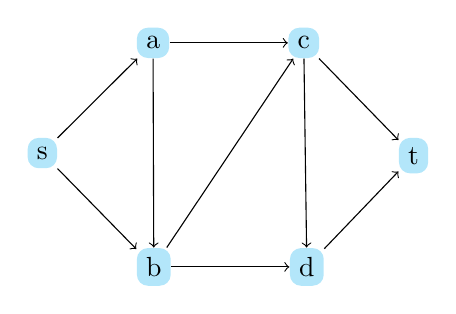
\begin{tikzpicture}[every node/.style={rectangle,fill=cyan!30,rounded corners}]
    \node (s) {s};
    \node[above right=of s] (a) {a};
    \node[below right=of s] (b) {b};
    \node[right=1.5cm of a] (c) {c};
    \node[right=1.5cm of b] (d) {d};
    \node[below right=of c] (t) {t};

    \foreach \u / \v in {s/a,s/b,a/b,a/c,b/c,b/d,c/d,c/t,d/t}
        \draw[->] (\u) -- (\v);
\end{tikzpicture}

\end{document}